\begin{flushleft}
\part{Versuche}

\section{Übersicht}

\subsection{Laboreinrichtung}


hier Foto von Versuchsaufbau allgemein, mit den drei Maschinen

\subsection{Maschinensatz}








\begin{tabular}{|L{5cm}|l|c|c|c|c|}
 \hline
 \rowcolor[gray]{.8} \textbf{$Bez.$} & \textbf{$P_{Nenn}$} & \textbf{$p$} & \textbf{$f$} & \textbf{$Spannung$ $\Delta$ / $Y$} & \textbf{$n_{Nenn}$}  \\
 \hline
Synchronmaschine&8.7 kW &2 &50 Hz&220/380 V&1500 $\frac{1}{min}$\\
\hline
Gleichstrommaschine&8.5 kW & - & - & 220 VDC& 1500 $\frac{1}{min}$\\
\hline
Schleifring ASM &10 kW &2&50 Hz& 230/400 V& 1420 $\frac{1}{min}$\\
\hline

\end{tabular}






\subsection{Messeinrichtungen}




\begin{tabular}{|L{0.8 \textwidth}|l|}
 \hline
 \rowcolor[gray]{.8} \textbf{Bezeichnung} & \textbf{Nr}  \\
 \hline
 Messtrennverstärker 1  & ET11002  \\
\hline
Messtrennverstärker 2  & ET11006  \\
\hline
Amperezange kleine Ströme & 431  \\
\hline
Amperezange grpsse Ströme & 544  \\
\hline
Oszilloskop  & 525  \\
\hline
Multimeter  & S20  \\
\hline
Drehzahl-und Drehmomentmessung  & 210  \\
\hline
Dreiphasiges Leistungsmessgerät PM 3000  & ET11071  \\
\hline
Synchronoskop   & 211  \\
\hline
\end{tabular}




\subsection{Speisungen und Belastungen}

\begin{tabular}{|L{0.3 \textwidth}|l|}
 \hline
 \rowcolor[gray]{.8} \textbf{Bezeichnung} & \textbf{Anwendungszweck}  \\
 \hline
 Chopper  & zur Erregung der SM  \\
\hline
Kastenwiderstand & Belastung ohmsch  \\
\hline
 Variac Einrichtung & Belastung reaktiv  \\
\hline

\end{tabular}



\newpage
\section{Inbetriebsetzung}
Als erstes sollen die Gleichstrommaschine sowie die ASM in Betrieb genommen werden und für die folgenden Messungen eingestellt werden.
\subsection{Gleichstrommaschine}
Die GM wird so eingestellt, dass sie beim Einschalten auf eine Drehzahl von 1500 $\frac{1}{min}$ hochfährt. Dies entspricht gerade der Nenndrehzahl der SM.

\subsection{ASM}
Die Asynchronmaschine wird im späteren Verlauf als Dämpfung für den SM genutzt. 
Da es sich um eine Schleifringläufer ASM handelt, kann über den Rotorkreis ein Widerstand zugeschalten werden. Dieser begrenzt den Anlaufstrom. Nach dem Hochfahren werden die Schleifringe kurzgeschlossen und die ASM kann als Kurzschlussläufer betrachtet werden.
\begin{figure}[H]
    \centering
        \includegraphics[ trim=0cm 11cm 0cm 4.5cm,
         clip, width=\textwidth]{DSCN2903}
    \caption{Übersicht der Maschinen SM (l), GM (m) und ASM (r)}
    \label{fig:Maschinenuebersicht}
\end{figure}


\newpage



\section{Maschinenkennwerte}\label{maschinenkennwerte}
In diesem Abschnitt werden die charakteristischen Kennwerte der SM ermittelt.

\subsection{Leerlaufkennlinie}
Mit der Leerlaufkennlinie wird der Zusammenhang der induzierten Phasenspannung (Effektivwert) in Abhängigkeit des Erregerstroms dargestellt. Für diesen Versuch muss die SM mit der Gleichstrommaschine bei Nenndrehzahl gehalten werden (1500 $\frac{1}{min}$).
Da die SM unbelastet ist, fliesst kein Strom $I_1$ durch die Statorwicklung, $\Delta U$ beträgt 0 und die Polradspannung (induzierte Spannung) entspricht der Phasenspannung $U_1$ resp. $U_{ph}$. \\


\begin{figure}[H]
    \centering
        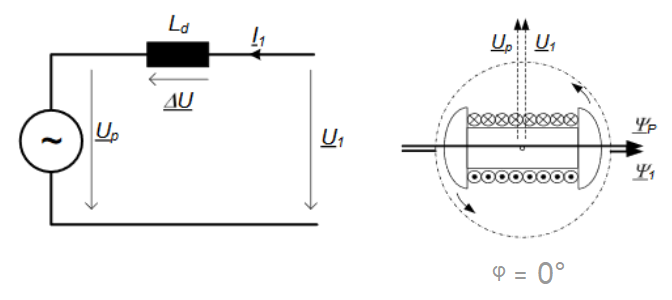
\includegraphics[ %trim=0.5cm 0.5cm 0.5cm 0.5cm,
         scale = 0.7]{leerlauf}
         \caption[Leerlaufbetrieb]{Leerlaufbetrieb \footnotemark}
    \label{fig:Leerlaufbetrieb}
\end{figure}

\footnotetext{Aus dem Skript 'Leistungselektronik und elektrische Antriebe' Kapitel 'Drehfeldmaschinen'}




\begin{figure}[H]
    \centering
        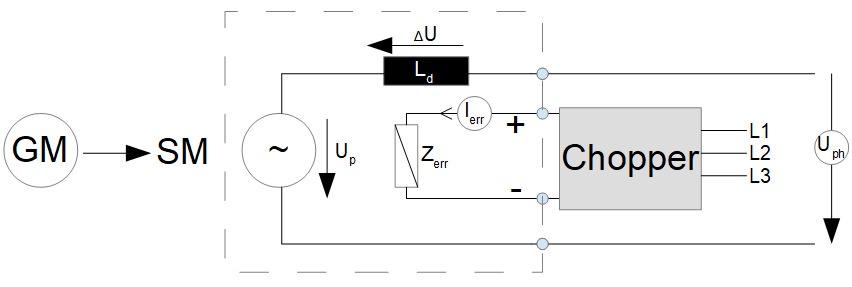
\includegraphics[ %trim=0.5cm 0.5cm 0.5cm 0.5cm,
         scale = 0.6]{leerlauf_schema}
    \caption{Schaltungsaufbau im VZS}
    \label{fig:Schaltungsaufbau}
\end{figure}









\newpage



\begin{figure}[H]
    \centering
        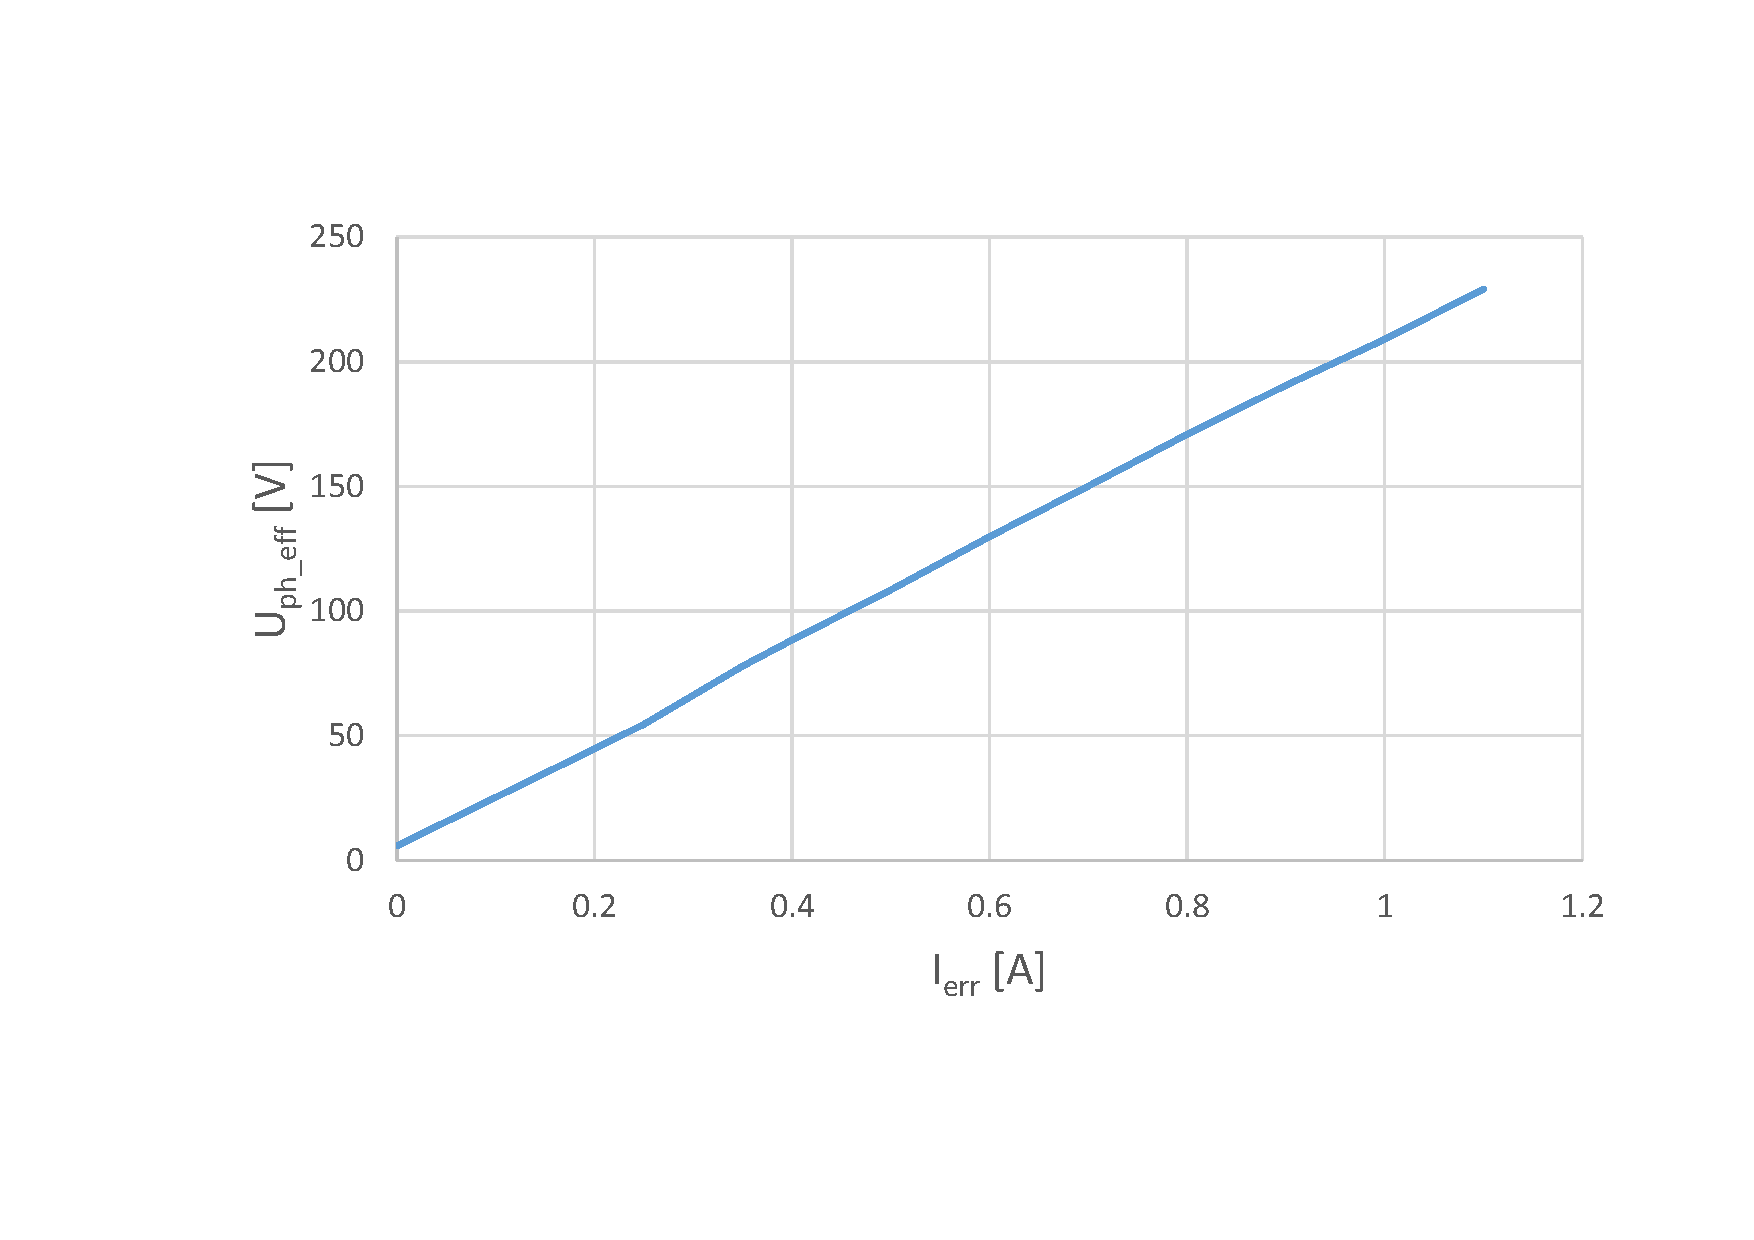
\includegraphics[ %trim=0.5cm 0.5cm 0.5cm 0.5cm,
         width=0.80\textwidth]{versuch_Uph_I_err.pdf}
    \caption{Phasenspannung in Abhängigkeit des Erregerstroms}
    \label{fig:Leerlaufkennlinie}
\end{figure}



Der Grafik ist zu entnehmen, dass die Phasenspannung durch das Erhöhen des Erregerstroms linear zunimmt. 
Die Kennlinie entspricht der Magnetisierungskennlinie der Synchronmaschine.\\


\vspace{0.4cm}
\textbf{Verwendete Messwerkzeuge}: Multimeter ($I_{err}$), Oszilloskop und\\ Messtrennverstärker 1($U_{ph}$)

\newpage






\subsection{Kurzschlusskennlinie}

Im Kurzschlussfall($U_1$ = 0V) fällt die induzierte Spannung $U_p$ über der Statorwicklung $\Delta U$ ab. Abhängig vom Erregerstrom verändert sich die induzierte Spannung und somit auch der Phasenstrom $I_1$ resp. $I_{ph}$.
Mit der Kurzschlusskennlinie soll dieser Zusammenhang grafisch dargestellt werden.
Auch in diesem Aufbau wird die SM mit der Gleichstrommaschine bei der Nenndrehzahl   betrieben.\\

\vspace{1cm}
 
 
\begin{figure}[H]
    \centering
        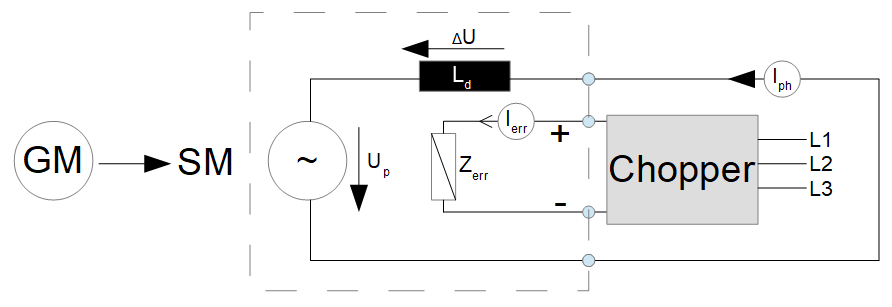
\includegraphics[ %trim=0.5cm 0.5cm 0.5cm 0.5cm,
         scale = 0.6]{kurzschluss_schema}
    \caption{Schaltungsaufbau im VZS}
    \label{fig:SchaltungsaufbauKurzschlusskennlinie}
\end{figure}



\begin{figure}[H]
    \centering
        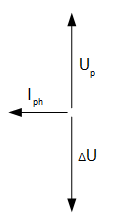
\includegraphics[ %trim=0.5cm 0.5cm 0.5cm 0.5cm,
         scale = 0.8]{zps_kurzschluss}
    \caption{Zeigerdiagramm im VZS}
    \label{fig:ZeigerdiagrammKurzschlusskennlinie}
\end{figure}


\begin{figure}[H]
    \centering
        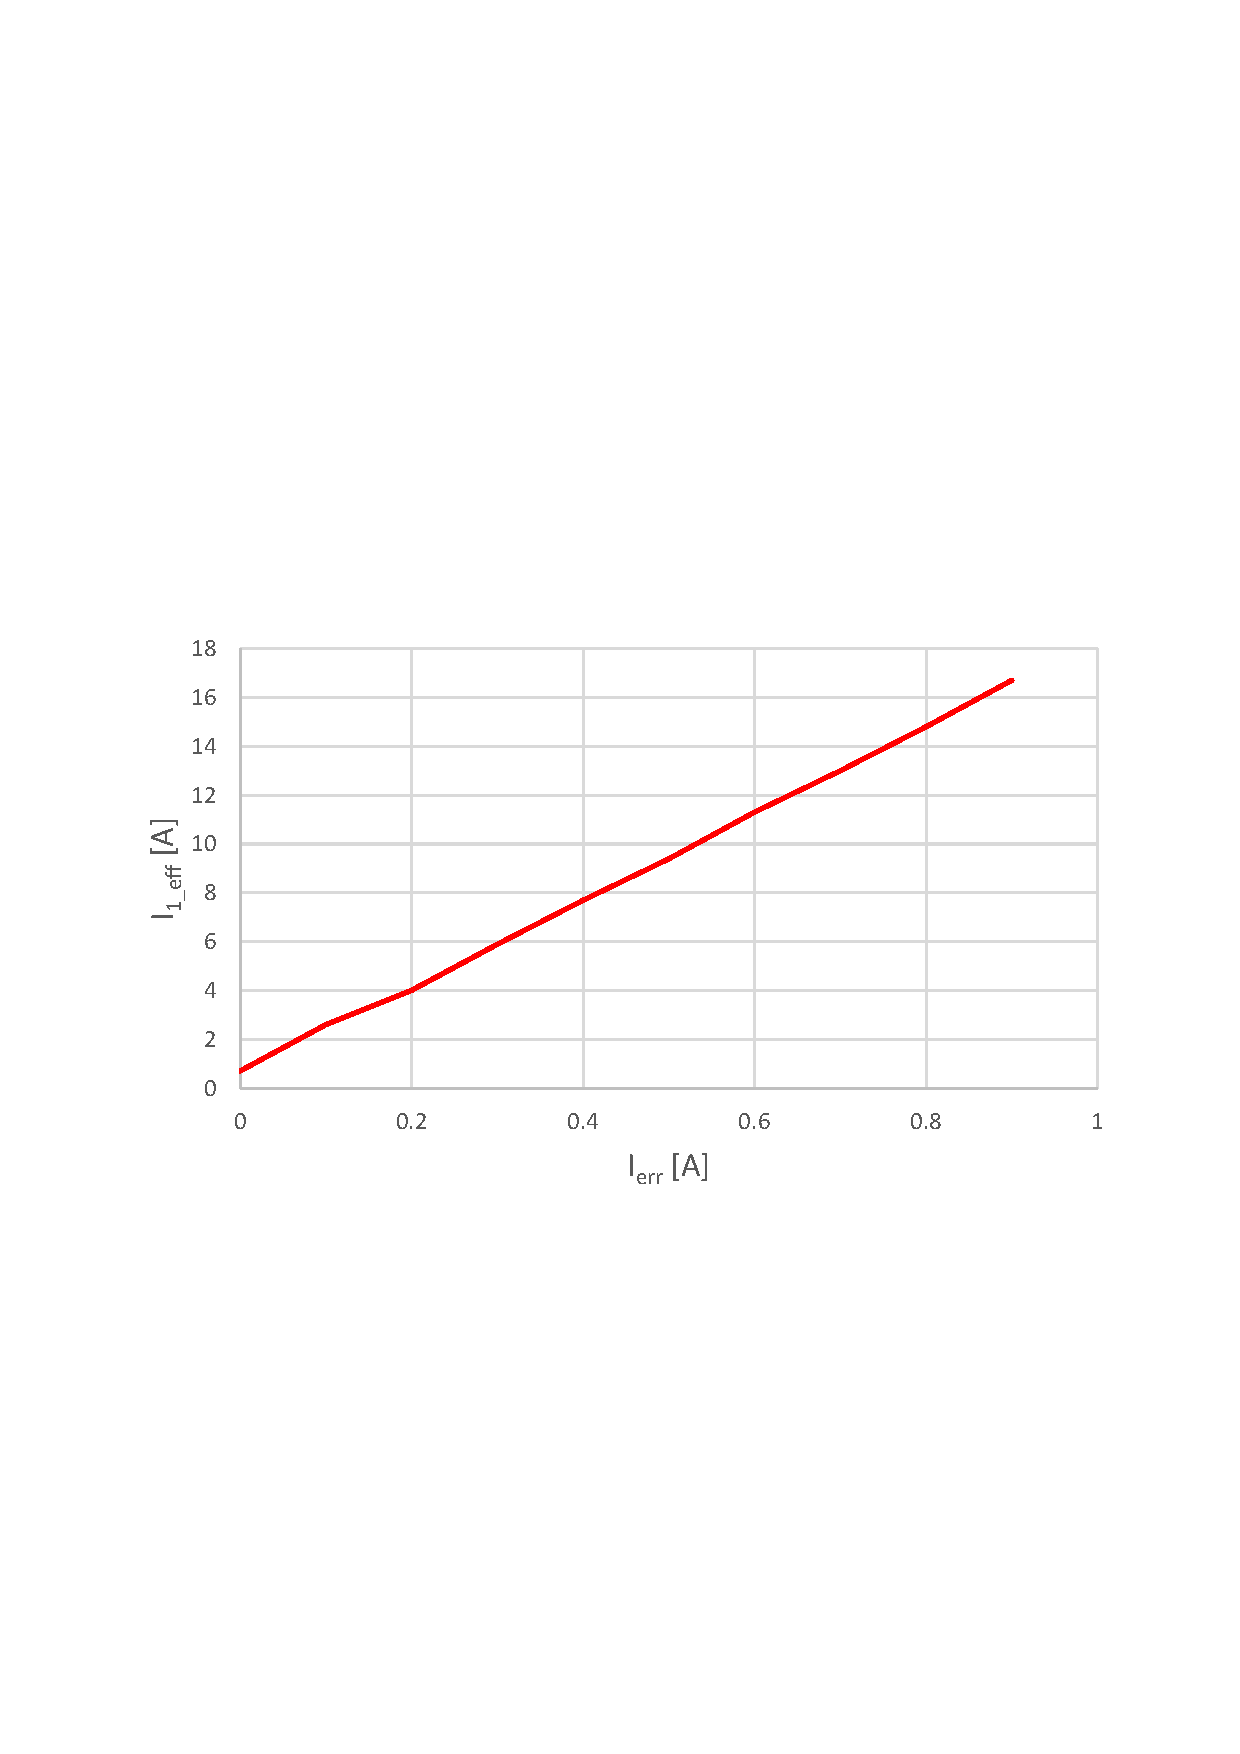
\includegraphics[ %trim=0.5cm 0.5cm 0.5cm 0.5cm,
         width=0.80\textwidth]{versuch_I_ph_I_err.pdf}
    \caption{Phasenstrom in Abhängigkeit des Erregerstroms}
    \label{fig:Kurzschlusskennlinie}
\end{figure}

Auch die Kurzschlusskennlinie verhält sich linear. Der Effektivwert des Phasenstroms nimmt proportional zum Erregerstrom zu.\\

\vspace{0.4cm}
\textbf{Verwendete Messwerkzeuge}: Multimeter ($I_{err}$), Oszilloskop und Amperezange($I_{ph}$) 




\newpage
\subsection{Längsreaktanz $X_d$}

Anhand der Messresultat vom Leerlauf-resp. Kurzschlussversuch lässt sich die Längsreaktanz $X_d$ berechnen. Da die SM mit der Nenndrehzahl betrieben wurde, dreht sich der Rotor mit der selben Winkelgeschwindigkeit wie das Statordrehfeld. In diesem Betriebsfall kann entsprechend nur die Längsreaktanz bestimmt werden.\\

Es gilt:\\

\vspace{0.3cm}
$$\underline{\Delta U} = j \cdot X_d \cdot \underline{I_1}$$
resp:\\
\vspace{0.3cm}
$$ X_d = \frac{\underline{\Delta U}}{j \cdot \underline{I_1}}  = 2 \cdot \pi \cdot f \cdot L_d$$\\

\vspace{0.5cm}


Im Leerlauffall gilt unter Vernachlässigung des Wicklungswiderstands vom Stator \\$\Delta U$ = $\underline{U_{1}}$. \\
Der Phasenstrom $I_1$ kann, bei selbem Erregerstrom, der Kennlinie beim Kurzschlussversuch entnommen werden. Für einen Erregerstrom von 0.4A ergibt sich:\\
\vspace{0.3cm}
\begin{itemize}
\item $\underline{U_{ph_eff}} = \Delta U = $ 150 V
\item $\underline{I_{1_eff}} = $ 8 A
\end{itemize}


und somit:

$$\underline{\underline{L_d}} = \frac{150 V }{j \cdot 8 A \cdot 2 \cdot \pi \cdot 50 Hz} = \underline{\underline{59.7 mH}}$$

\newpage



\subsection{Schwebeverfahren} \label{schwebeverfahren}
Zur Ermittlung der Längs -und Querreaktanz wird in diesem Versuch das Schwebeverfahren angewendet. Dazu wird die SM über die Gleichstrommaschine mit einem kleinen Schlupf betrieben. Gleichzeitig wird der Stator der SM mit reduzierter Spannung (Variac) gespeist. Die Erregerwicklung wird für diesen Versuch nicht betrieben.\\
\vspace{0.4cm}


 \begin{figure}[H]
    \centering
        \includegraphics[ %trim=0.5cm 0.5cm 0.5cm 0.5cm,
         scale = 0.45]{Schwebeverfahren}
    \caption{Schaltungsaufbau im VZS}
    \label{fig:SchaltungsaufbauSchwebeverfahren}
\end{figure}


Die Phasenspannung am Stator wurde mit dem Variac auf einen Effektivwert von ungefähr 50V gedrosselt (Abbildung 8). 


\begin{figure}[H]
    \centering
        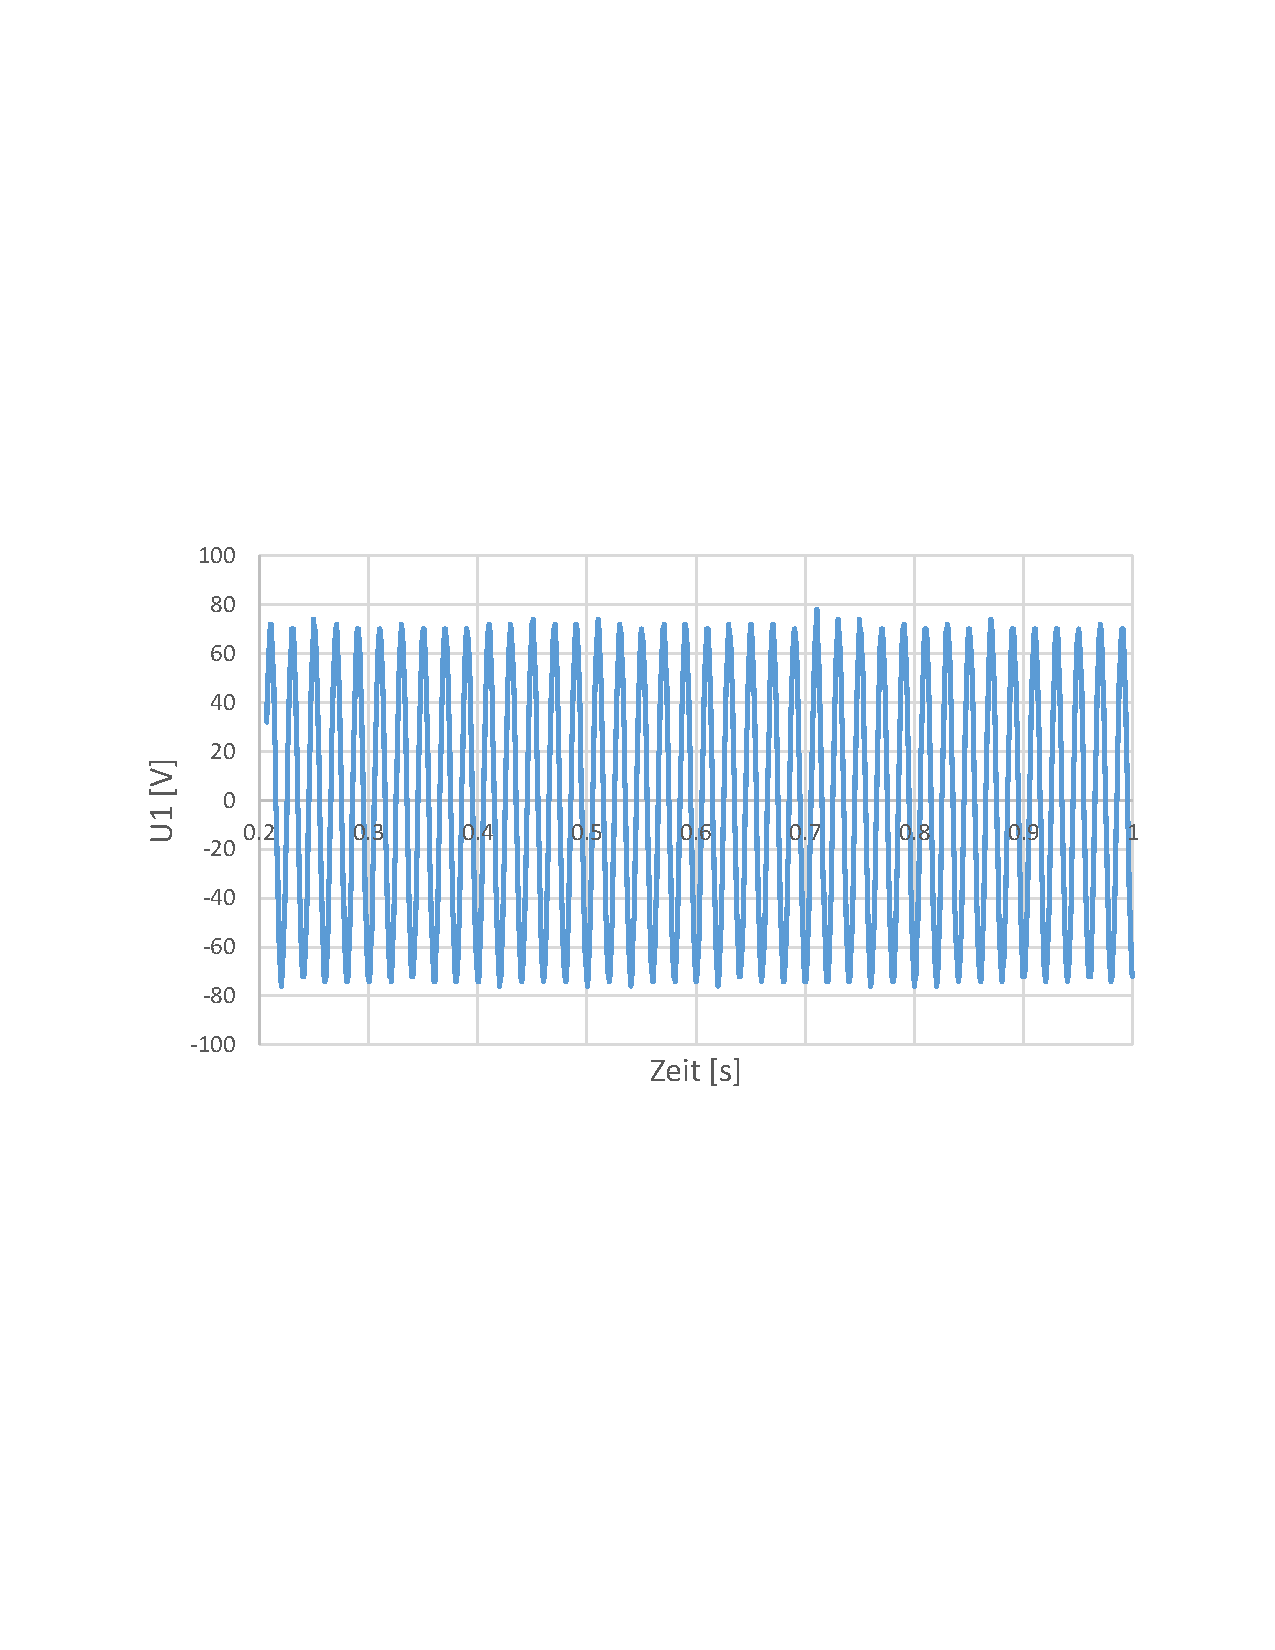
\includegraphics[ trim=0.5cm 9cm 0.5cm 9cm,
         width=1\textwidth]{schwebeverfahren_U_1.pdf}
    \caption{Phasenspannung $U_1$ resp $U_{ph}$}
    \label{fig:PhasenspannungSchwebeverfahren}
\end{figure}


\newpage

Der zugehörige Phasenstrom:\\
\vspace{0.3cm}
\begin{figure}[H]
    \centering
        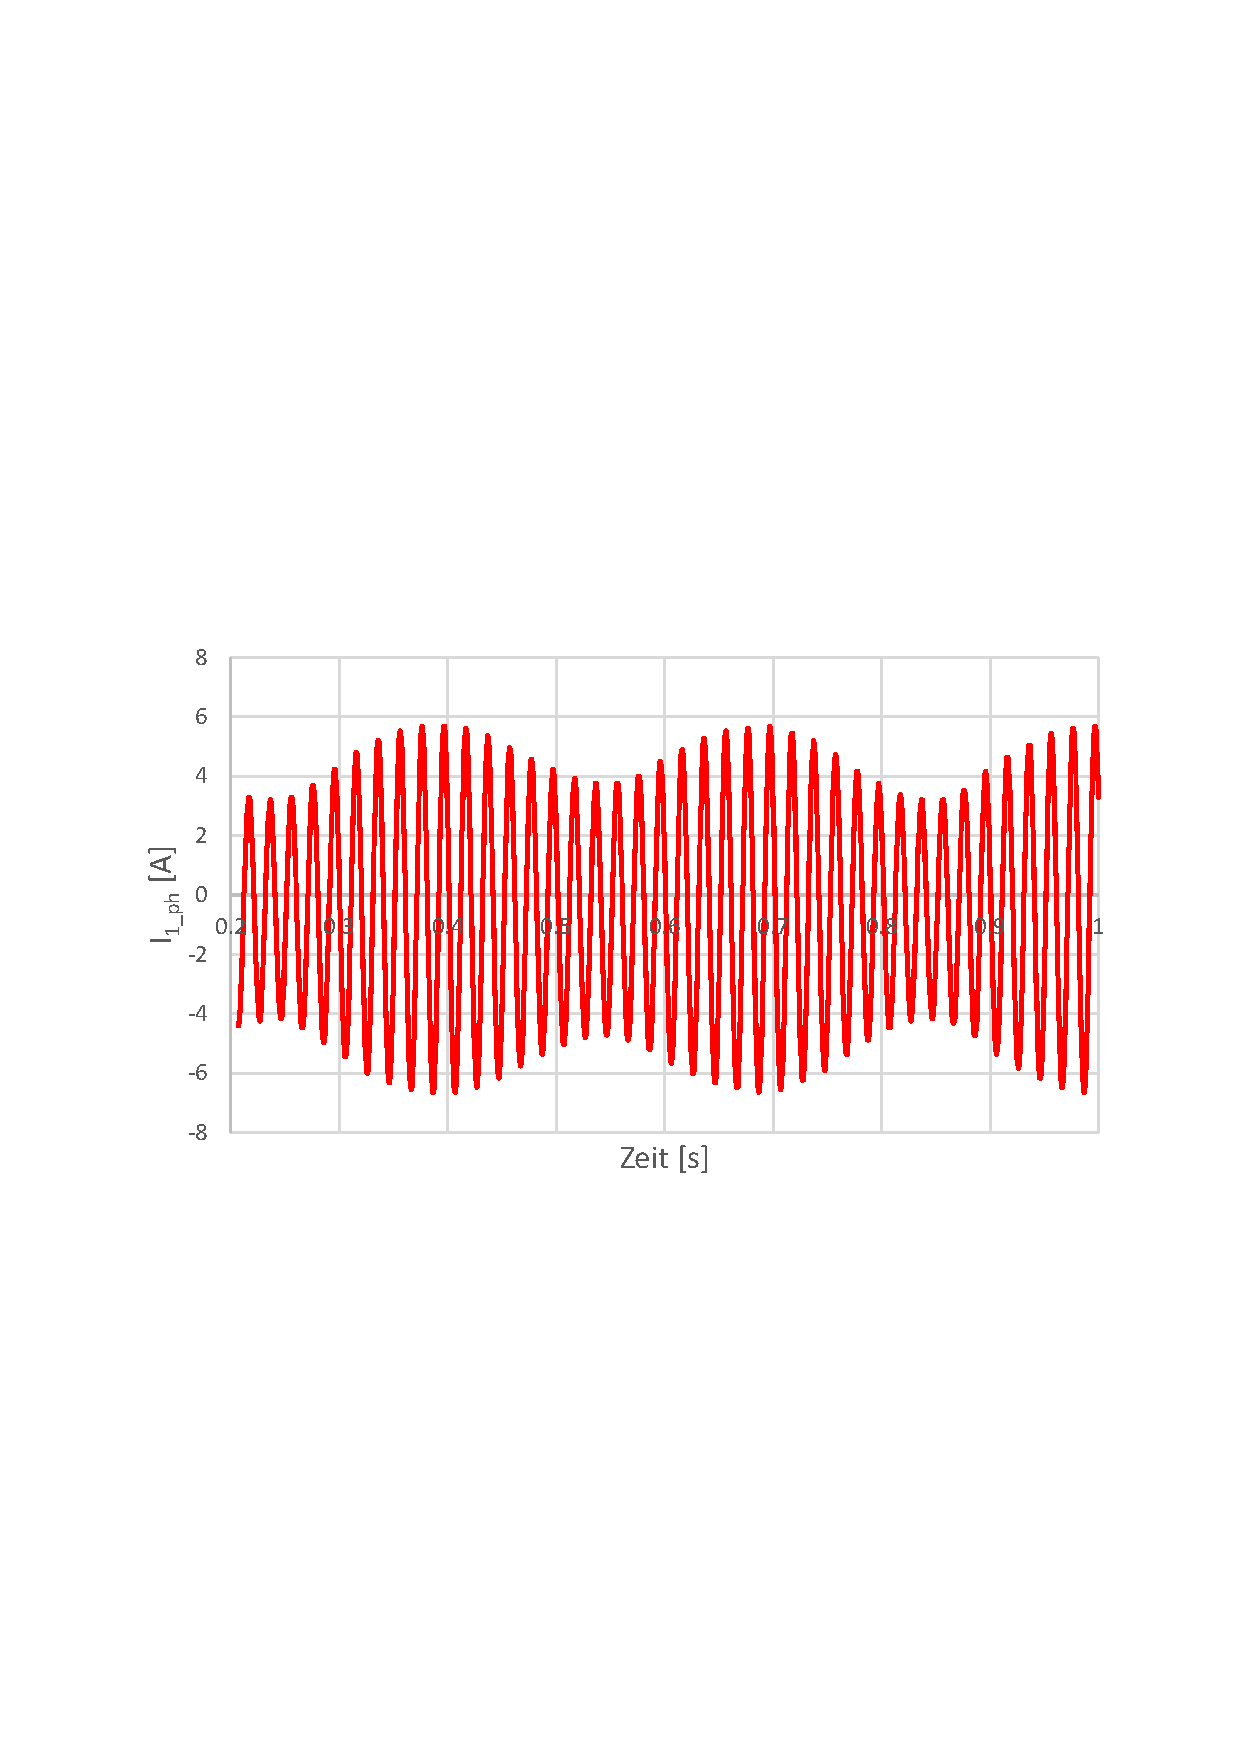
\includegraphics[% trim=0.5cm 9cm 0.5cm 9cm,
         width=0.8\textwidth]{schwebeverfahren_I_ph.pdf}
    \caption{Phasenstrom $I_1$ resp $I_{ph}$}
    \label{fig:PhasenstromSchwebeverfahren}
\end{figure}


Da die Polradspannung $U_p$ beim Schwebeverfahren 0V beträgt, fällt die gesamte Spannung $U_1$ über der Impedanz der Maschine ab. 
Zur Bestimmung der Längsreaktanz $X_d$, resp. Querreaktanz $X_q$ wird der Verlauf des Phasenstroms betrachtet (Abbildung 9).\\
\vspace{0.4cm}

\underline{Längsreaktanz}\\
\vspace{0.2cm}
Die Längsreaktanz wird zum Zeitpunkt, wenn der Strom $I_1$ minimal ist  berechnet (zb. t = 0,55s). 
Durch einsetzen des magnetischen Fluss $\Phi$, gleichgesetzt mit der Summe der Ströme in der Spule $N*I$, in die Induktionsgleichung für die Spannung $u$, kann gezeigt werden, dass die Induktivität $L$ bei kleinem Luftspalt gross wird. Bei gleichbleibender Spannung muss also der Strom $I$ beim kleinsten Luftspalt minimal sein. 


\begin{center}
\begin{Large}
$ \underline{\underline{L_d}}= \frac{\frac{\hat{U}_1}{\sqrt{2}}}{j \cdot 2 \cdot \pi \cdot f \cdot \frac{\hat{I}_{ph}}{\sqrt{2}} }  = \frac{\frac{75 V}{\sqrt{2}}}{j \cdot 2 \cdot \pi \cdot 50 \cdot \frac{3.9 A}{\sqrt{2}} } = \underline{\underline{61 mH}}$\\
\end{Large}
\end{center}


\newpage




\underline{Querreaktanz}\\
\vspace{0.2cm}
Umgekehrt wird die Querreaktanz zum Zeitpunkt, wenn die Induktivität minimal und somit der Strom maximal ist berechnet (zb. t = 0,7s). Hier ist der Luftspalt am grössten.

\begin{center}
\begin{Large}
$ \underline{\underline{L_q}}= \frac{\frac{\hat{U}_1}{\sqrt{2}}}{j \cdot 2 \cdot \pi \cdot f \cdot \frac{\hat{I}_{ph}}{\sqrt{2}} }  = \frac{\frac{75 V}{\sqrt{2}}}{j \cdot 2 \cdot \pi \cdot 50 \cdot \frac{5.8 A}{\sqrt{2}} } = \underline{\underline{41 mH}}$\\
\end{Large}
\end{center}


\vspace{0.4cm}
\textbf{Verwendete Messwerkzeuge}:  Oszilloskop, Amperezange($I_{ph}$),\\ Messtrennverstärker 1 ($U_{ph}$) 


\newpage
\section{SM als Generator im Inselbetrieb}\label{inselbetrieb}
\subsection{Belastungskennlinie}
Bei diesem Versuch wirkt die Synchronmaschine als Generator im Inselbetrieb. Die Gleichstrommaschine dient als Antrieb.
\vspace{0.3cm}
\begin{figure}[H]
    \centering
        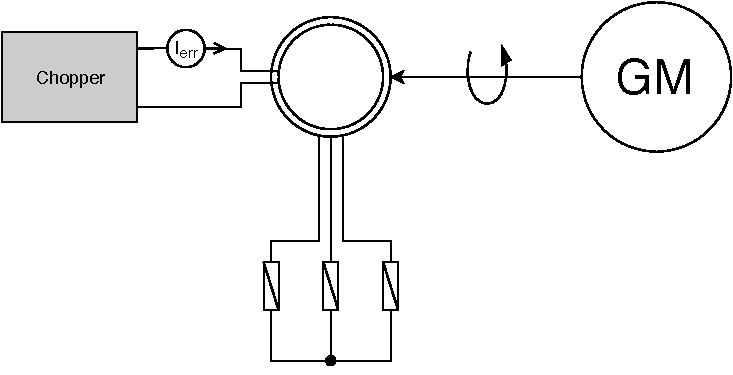
\includegraphics[ %trim=1cm 16.5cm 7.6cm 5.7cm,clip,
         width=0.8\textwidth]{SM_Inselbetrieb_Uebersicht.pdf}
    \caption{Übersicht SM im Inselbetrieb}
    \label{fig:SMInselbetrieb}
\end{figure}
\vspace{0.3cm}
Bei konstantem  Erregerstrom und konstanter Drehzahl wird die Phasenspannung $U_1$, der Phasenstrom $I_1$ und der Polradwinkel $\vartheta$ bei verschiedenen Lasten gemessen. Zum einen werden die Daten bei einer kapazitiven, einer induktiven und einer ohmschen Last jeweils mit $I_{1_{eff}}$ resp. $I_{ph_{eff}}$ = 4.8A gemessen.

\begin{itemize}
\item \makebox[5cm][l]{$I_{err} = $ 1.1 A  }            konstanter Erregerstrom
\item \makebox[5cm][l]{$n =  1500 \frac{1}{min}$}				konstante Drehzahl
\end{itemize}
%\newpage


Zuerst wurde die SM in den Leerlaufbetrieb versetzt um die Polradspannung bei einem Erregerstrom von 1.1 A zu ermitteln. Für $U_1$ resp. $U_{ph}$ konnte man so eine Spannung von 228V messen, dieser Wert kann für die Polradspannung $U_p$ bei den folgenden Betriebsarten verwendete werden. 

\subsubsection{Ohmsche Belastung}

\begin{figure}[H]
\begin{minipage}[t]{0.45\textwidth}
\centering
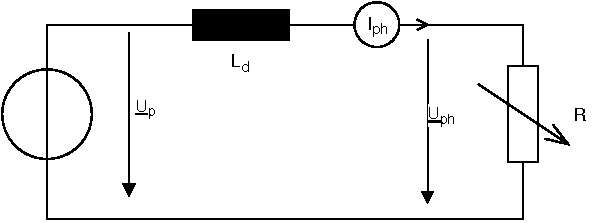
\includegraphics[width=\textwidth]{SM_Insel_1PH_R.pdf}
\subcaption{Schema ohmsche Last im EZS}
\label{fig:SM_Insel_1PH_R}
\end{minipage}
\begin{minipage}[t]{0.4\textwidth}
\centering
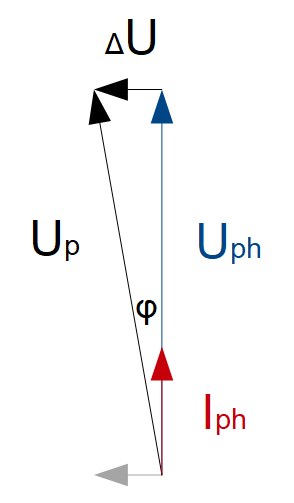
\includegraphics[width=0.4\textwidth]{631_zeiger_ohmsch}
\subcaption{Zeigerdiagramm im EZS}
    \label{fig:ZeigerR}
\end{minipage}
\end{figure}


\underline{Messresultate:}\\
\vspace{0.3cm}

\begin{itemize}
\item \makebox[5cm][l]{$\varphi = 6\degree$  }            Polradwinkel
\item \makebox[5cm][l]{$U_{ph_{eff}} = 223 V$   }         Effektivwert der Phasenspannung
\item \makebox[5cm][l]{$I_{ph_{eff}} = 4.85 A$   }        Effektivwert des Phasenstrom    
\end{itemize}

\vspace{0.5cm}

\begin{tabular}{|l|l|l|l|l|l|}
 \hline
 \rowcolor[gray]{.8} \textbf{Ermittlungsart} & \textbf{$U_1 [V]$}&   \textbf{$I_1 [A]$} &\textbf{$\Delta U [V]$} & \textbf{$U_p [V]$} & \textbf{$\varphi$}\\
 \hline
 Polradmessung mit Gleichungen~\ref{eq:Polradmessung}& $223$ & $4.85$ & 23.4& 224& $6\degree$ \\
\hline
 $\Delta U$ aus $L_q$ mit Gleichungen~\ref{eq:deltaU} & $223$ & $4.85$ & 62.5& 231.6& $15.6\degree$ \\
\hline
 $U_p$ aus Abbildung \ref{fig:Leerlaufkennlinie} mit Gleichungen~\ref{eq:Up} & $223$ & $4.85$ & 53& 229.2&  $13.4\degree$\\
\hline
\end{tabular}

Die Unterschiede sind auf die vernachlässigten ohmschen Verluste in den Maschinenwicklungen zurück zu führen. Das bedeutet, das $\Delta U$ nicht exakt $90\degree$ voreilend zu $I_1$ ist.
\begin{equ}[H]
\begin{equation} \label{eq:Polradmessung}
\begin{aligned}
 U_p = \frac{U_1}{cos(\varphi)} = 224 V \\
 \Delta U = \sqrt{U_p^2-U_1^2} = 23.4 V 
\end{aligned}
\end{equation}
\caption{Berechnungen mit dem gemessenen Polradwinkel}
\end{equ} 

\begin{equ}[H]
\begin{equation} \label{eq:deltaU}
\begin{aligned} 
	\Delta U = 2*\pi*f*L_q*I_1 = 62.5 V \\
	U_p = \sqrt{\Delta U^2+U_1^2} = 231.6 V \\
	\varphi = arccos(\frac{U_1}{U_p} = 15.6\degree)
	\end{aligned}
\end{equation} 
\caption{Berechnungen über die ermittelte Reaktanz}
\end{equ}

In der Berechnung wird $L_q$ verwendet, da der Strom $I_1$ bei ohmscher Last annähernd parallel zu $U_p$ verläuft und somit die q-Komponenten des Stromes den Haupteinfluss verursacht.

\begin{equ}[H]
\begin{equation} \label{eq:Up}
\begin{aligned} 
	U_p  = 229.2 V \\
	\Delta U = \sqrt{U_p^2-U_1^2} = 53 V \\
	\varphi = arccos(\frac{U_1}{U_p}) = 13.4\degree
	\end{aligned}
\end{equation} 
\caption{Berechnungen über die Leerlaufkennlinie}
\end{equ}



\begin{figure}[H]
    \centering
    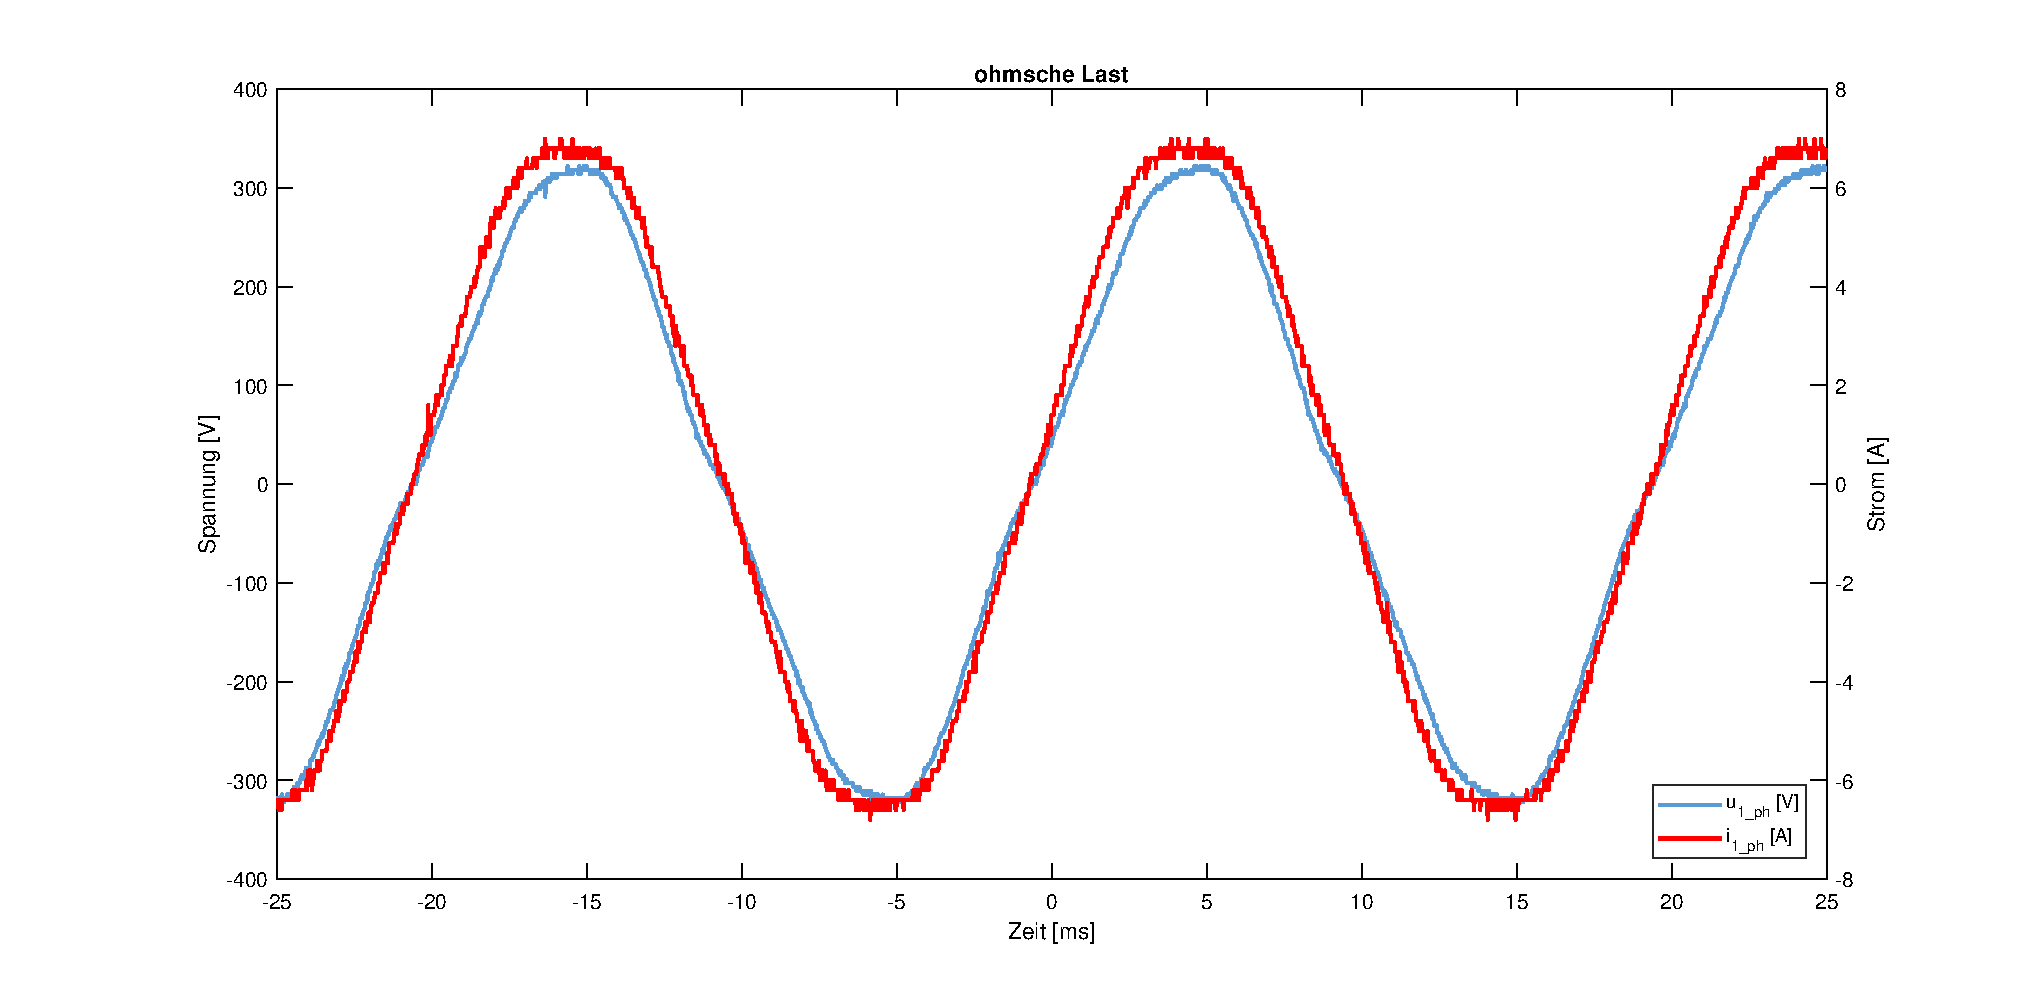
\includegraphics[width=\textwidth]{631_Ohmsch}
    \caption{Messung mit dem KO}
    \label{fig:U/I_R}
\end{figure}

%\textcolor{red}{@Andy: bisch ufs gliche cho? Zusätzlich noch begründen wiso Querreaktanz relevant ist -> gemacht! Verständlich?\\
%@Theo: Gleichung 1 ond Gleichung 2 beni of s glich echo ond  ech hätti d Abwichig au so begröndet. Aber d Glichig 3 esch mer ned ganz klar, resp. woher hesch die 397 Volt ? ok ha d Leerlaufkennlinie :P, aber wiso hesch dor worzle 3 grächnet ? esch demfall d Achsebeschreftig falsch ? well det hemmer ja au d Phasespannig gmässe - Phase zu Sternpunkt\\
%Theo: Bisch sicher? de isch si aber huärä höch und de würd d'Rächnig nid uf ga... hei mär dert nid Phase-Phase gmässä?\\
%Andy: Ja ech be äbe nöme secher, ha gmeint mer hend no disskutiert vo wo zo wo dassmer mässid (Abbildung 2) ond send zom entschloss cho, dasses zom Sternponkt gohd, obwohl es de eigendlech werkli kei senn macht :(\\
%Theo: s'Muäss eigändläch d'Phase-Phase-Spannig si. Omlin het sogar no gseit, mit den $I_e =1.1$ chöm mä öpä gad uf 230V $U_1$\\
%Andy: Ja esch guet, aber Phasespannig bedütet för mech Phas -> Sternponkt, dorom mössts denn wohl verkettete Spannung heisse bide Abbildung 2.\\
%Andere Frage: Bis wenn moss mer de Laborbrecht fertig ha ?\\
%Theo: Auso i glob 10 Tag nach em Versuech! Uaso am letzä Mänti... Iz isch dfrag ob mär nä hüt fertig mache oder ig am Omlin schribä das er bis am Friti bi im isch... I passe Abbiudig 2 a (i tuä eifach scho der aues dür sqrt{3} teilä...\\ Andy: ech wörd säge mer macheds bes am Fritig fertig, de chömmer morn no gschwend bespräche was mer no alles muess mache. Schriebsch du demfall im Omlin es Mail?}
%\newpage




\subsubsection{Kapazitive Belastung}

\begin{figure}[H]
\begin{minipage}[t]{0.65\textwidth}
\centering
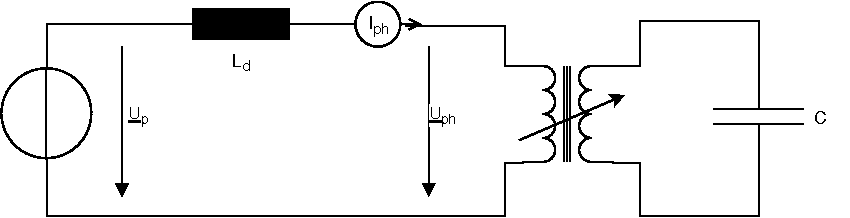
\includegraphics[width=\textwidth]{SM_Insel_1PH_C.pdf}
\subcaption{Schema kapazitive Last im EZS}
\label{fig:SM_Insel_1PH_C}
\end{minipage}
\begin{minipage}[t]{0.3\textwidth}
\centering
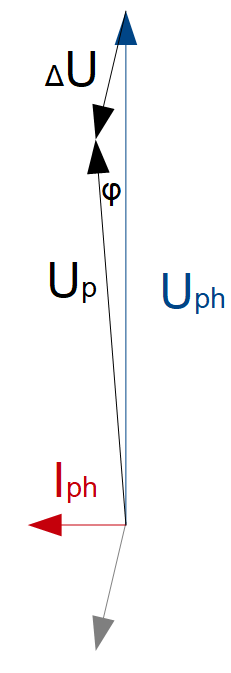
\includegraphics[width=0.3\textwidth]{631_zeiger_kap}
\subcaption{Zeigerdiagramm im EZS}
    \label{fig:ZeigerC}
\end{minipage}
\end{figure}


\underline{Messresultate:}\\
\vspace{0.3cm}


\begin{itemize}
\item \makebox[5cm][l]{$\varphi = 1.4\degree$  }            Polradwinkel
\item \makebox[5cm][l]{$U_{ph_{eff}} = 266 V$   }         Effektivwert der Phasenspannung
\item \makebox[5cm][l]{$I_{ph_{eff}} = 4.8 A$   }        Effektivwert des Phasenstrom    
\end{itemize}

\vspace{0.3cm}

\begin{figure}[H]
    \centering
    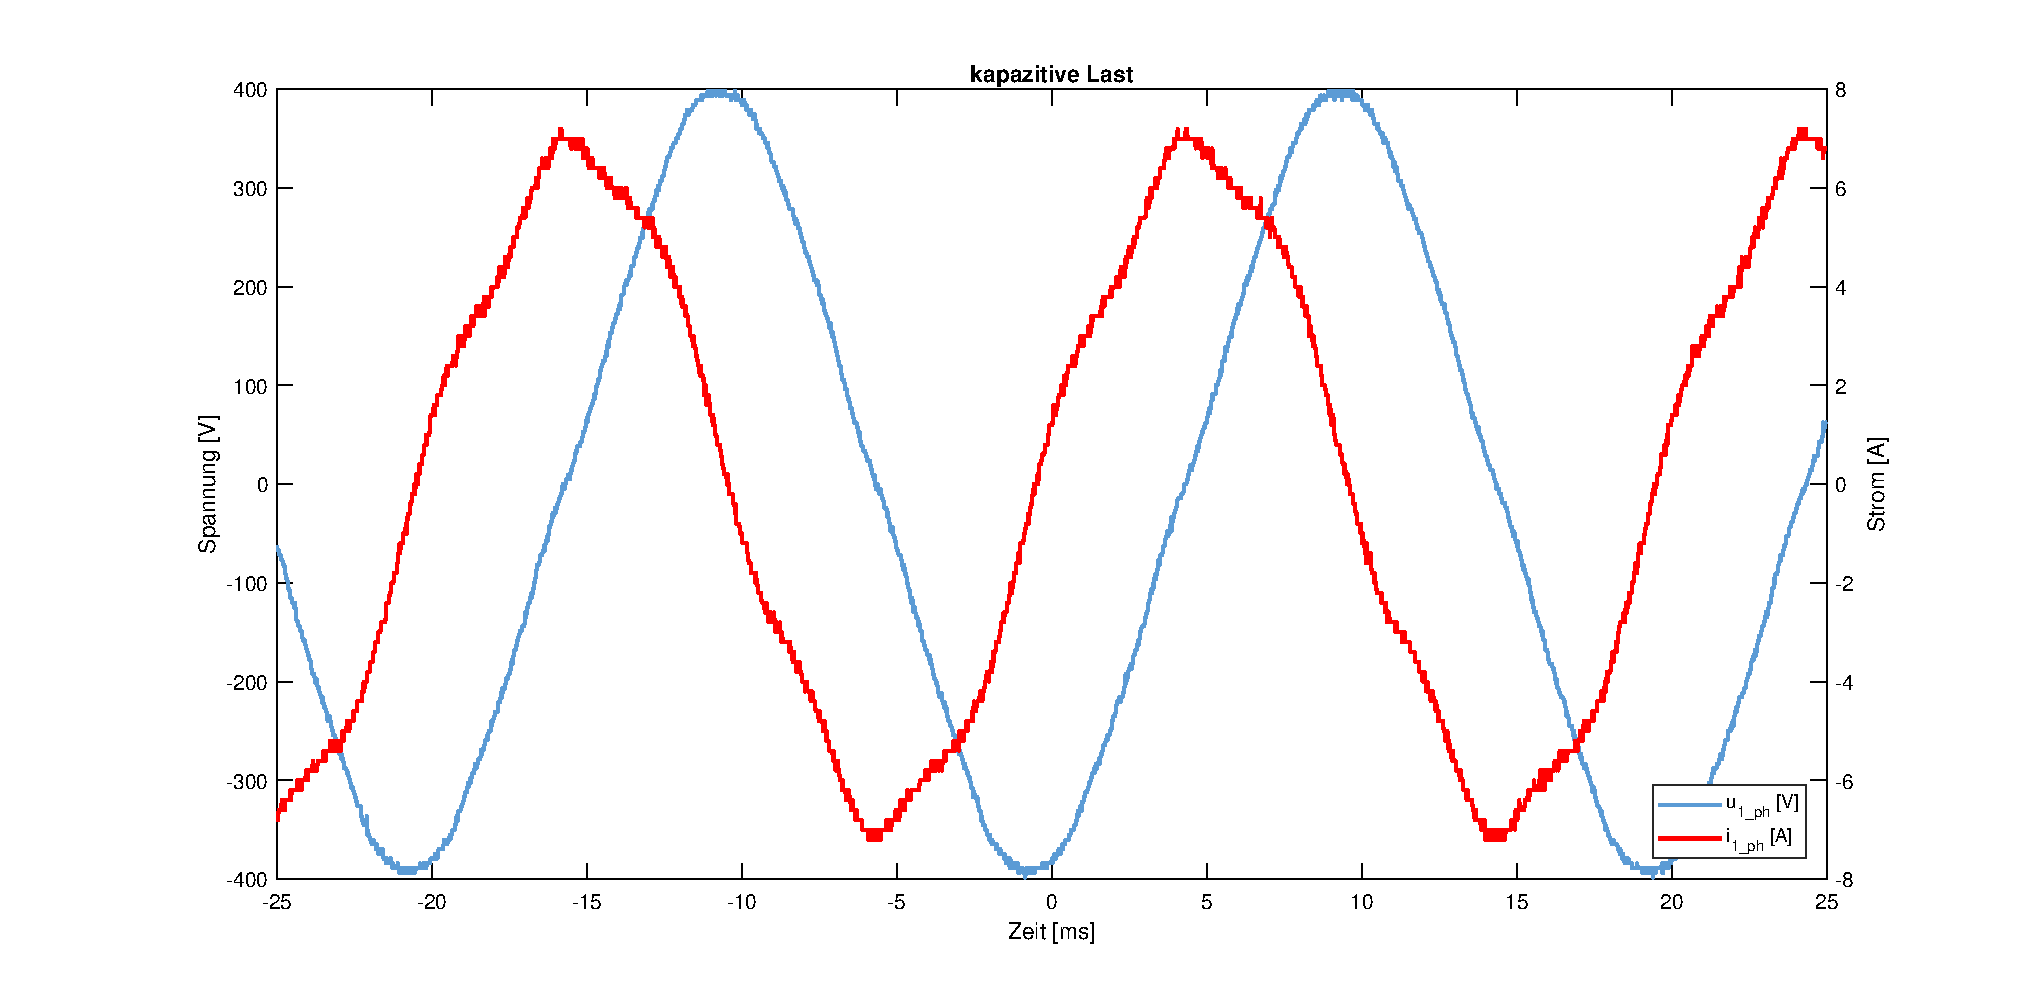
\includegraphics[width=0.9\textwidth]{631_Kapazitiv}
    \caption{Messung mit dem KO}
    \label{fig:U/I_C}
\end{figure}

An der Messkurve ist zu erkennen, dass der Phasenstrom der Phasenspannung um ca. 90 \degree voreilt. Weiter ist die erhöhte Phasenspannung gegenüber der ohmschen Last von der vorangehenden Messung ersichtlich. 









\newpage




\subsubsection{Induktive Belastung}

\begin{figure}[H]
\begin{minipage}[t]{0.65\textwidth}
\centering
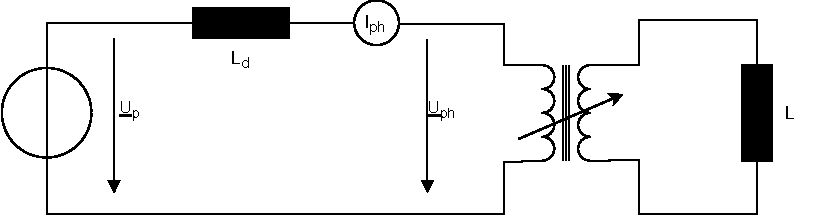
\includegraphics[width=\textwidth]{SM_Insel_1PH_L.pdf}
\subcaption{Schema induktive Last im EZS}
\label{fig:SM_Insel_1PH_L}
\end{minipage}
\begin{minipage}[t]{0.3\textwidth}
\centering
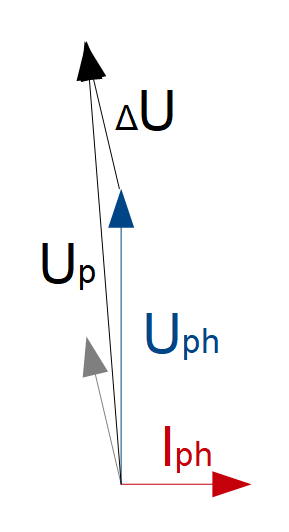
\includegraphics[width=0.5\textwidth]{631_zeiger_ind}
\subcaption{Zeigerdiagramm im EZS}
    \label{fig:ZeigerL}
\end{minipage}
\end{figure}


\underline{Messresultate:}\\
\vspace{0.3cm}


\begin{itemize}
\item \makebox[5cm][l]{$\varphi = 0.6\degree$  }            Polradwinkel
\item \makebox[5cm][l]{$U_{ph_{eff}} = 180 V$   }         Effektivwert der Phasenspannung
\item \makebox[5cm][l]{$I_{ph_{eff}} = 4.8 A$   }        Effektivwert des Phasenstrom    
\end{itemize}

\vspace{0.2cm}

\begin{figure}[H]
\centering
        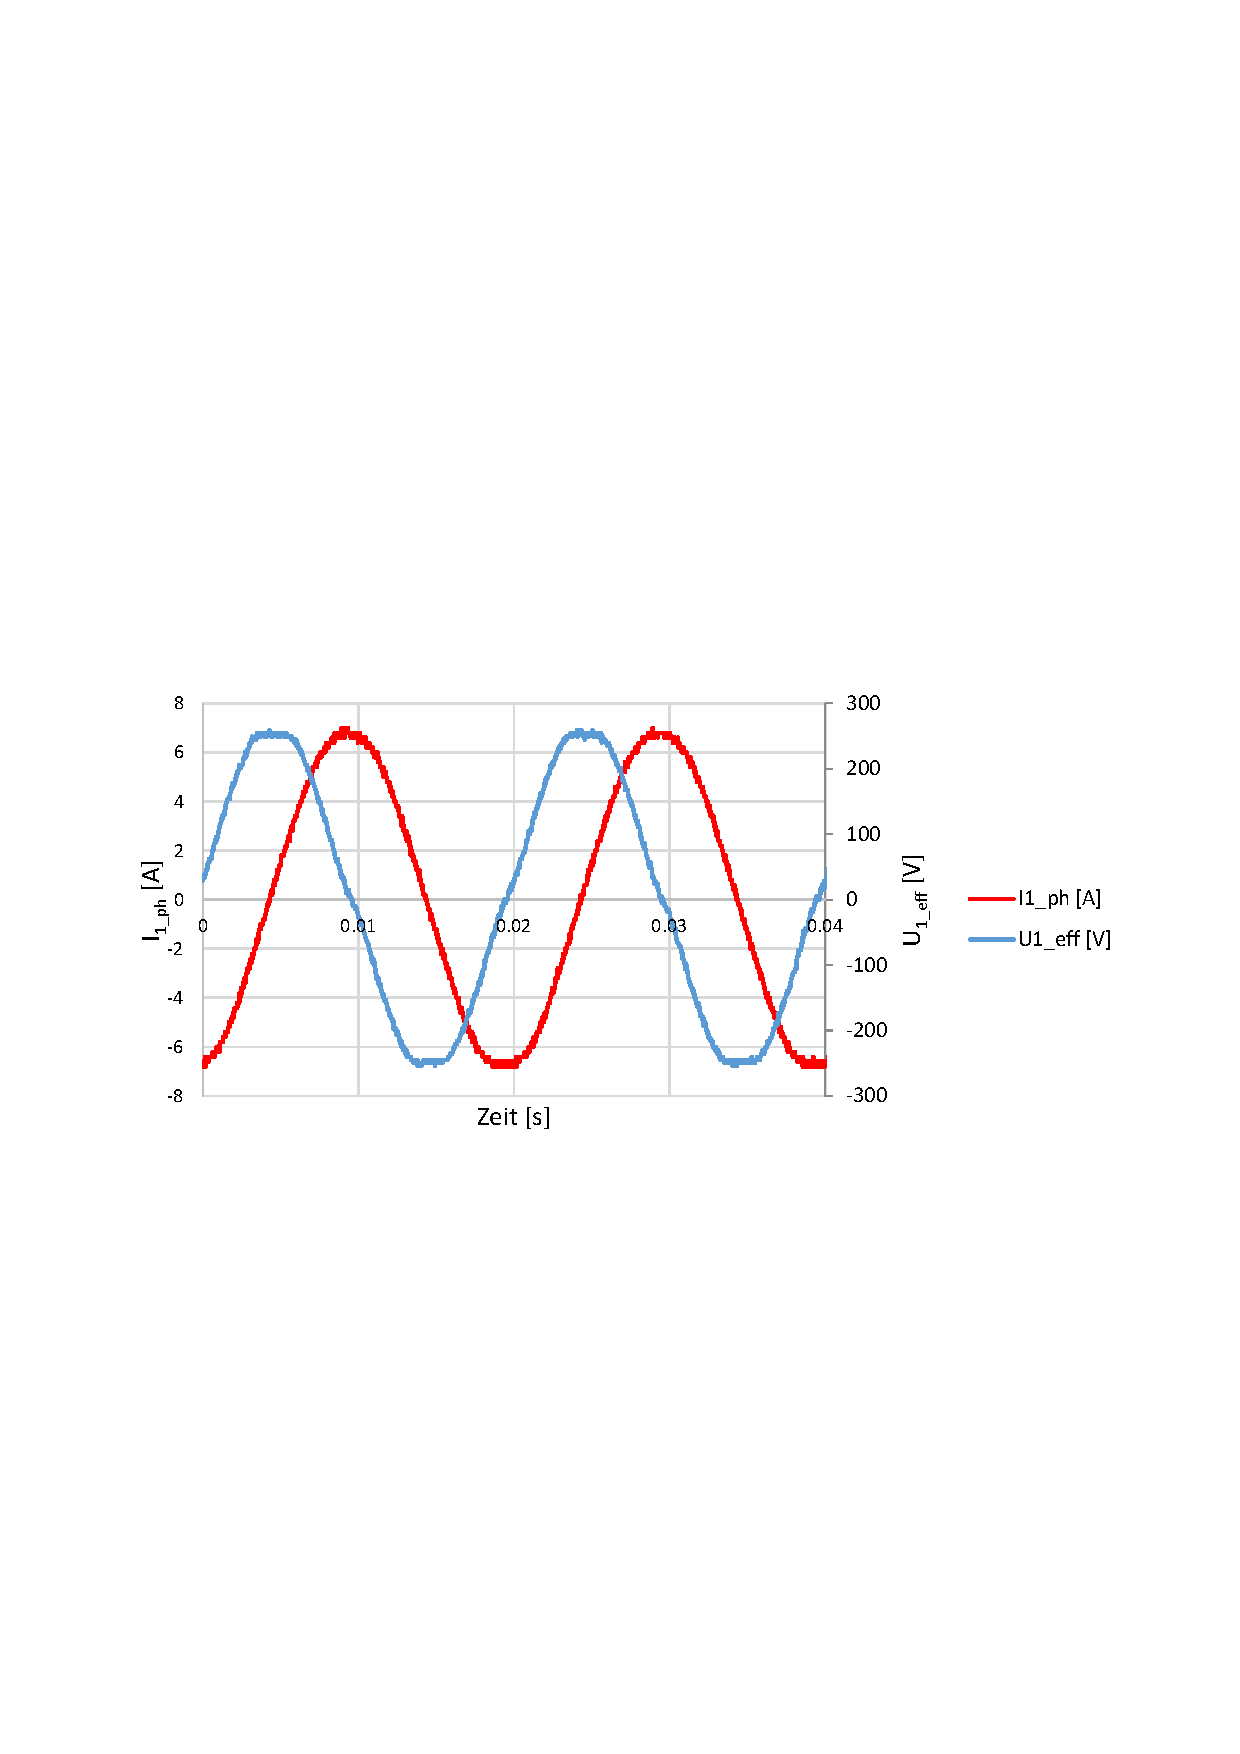
\includegraphics[ %trim=0.5cm 1cm 0.5cm 1cm,
        % width=0.8\textwidth]{631_Bild6_Induktiv.pdf}
				width=0.9\textwidth]{631_Induktiv}
    \caption{Messung mit dem KO}
    \label{fig:U/I_L}
\end{figure}

Die Phasenspannung eilt dem Phasenstrom um 90 \degree voraus. Auch hier ist der Einfluss der Belastungsimpedanz auf die Amplitude der Phasenspannung gut erkennbar. Während sie bei kapazitiver Last zunimmt, sinkt sie bei einer induktiven Belastung. \\

\begin{figure}[H]
    \centering
        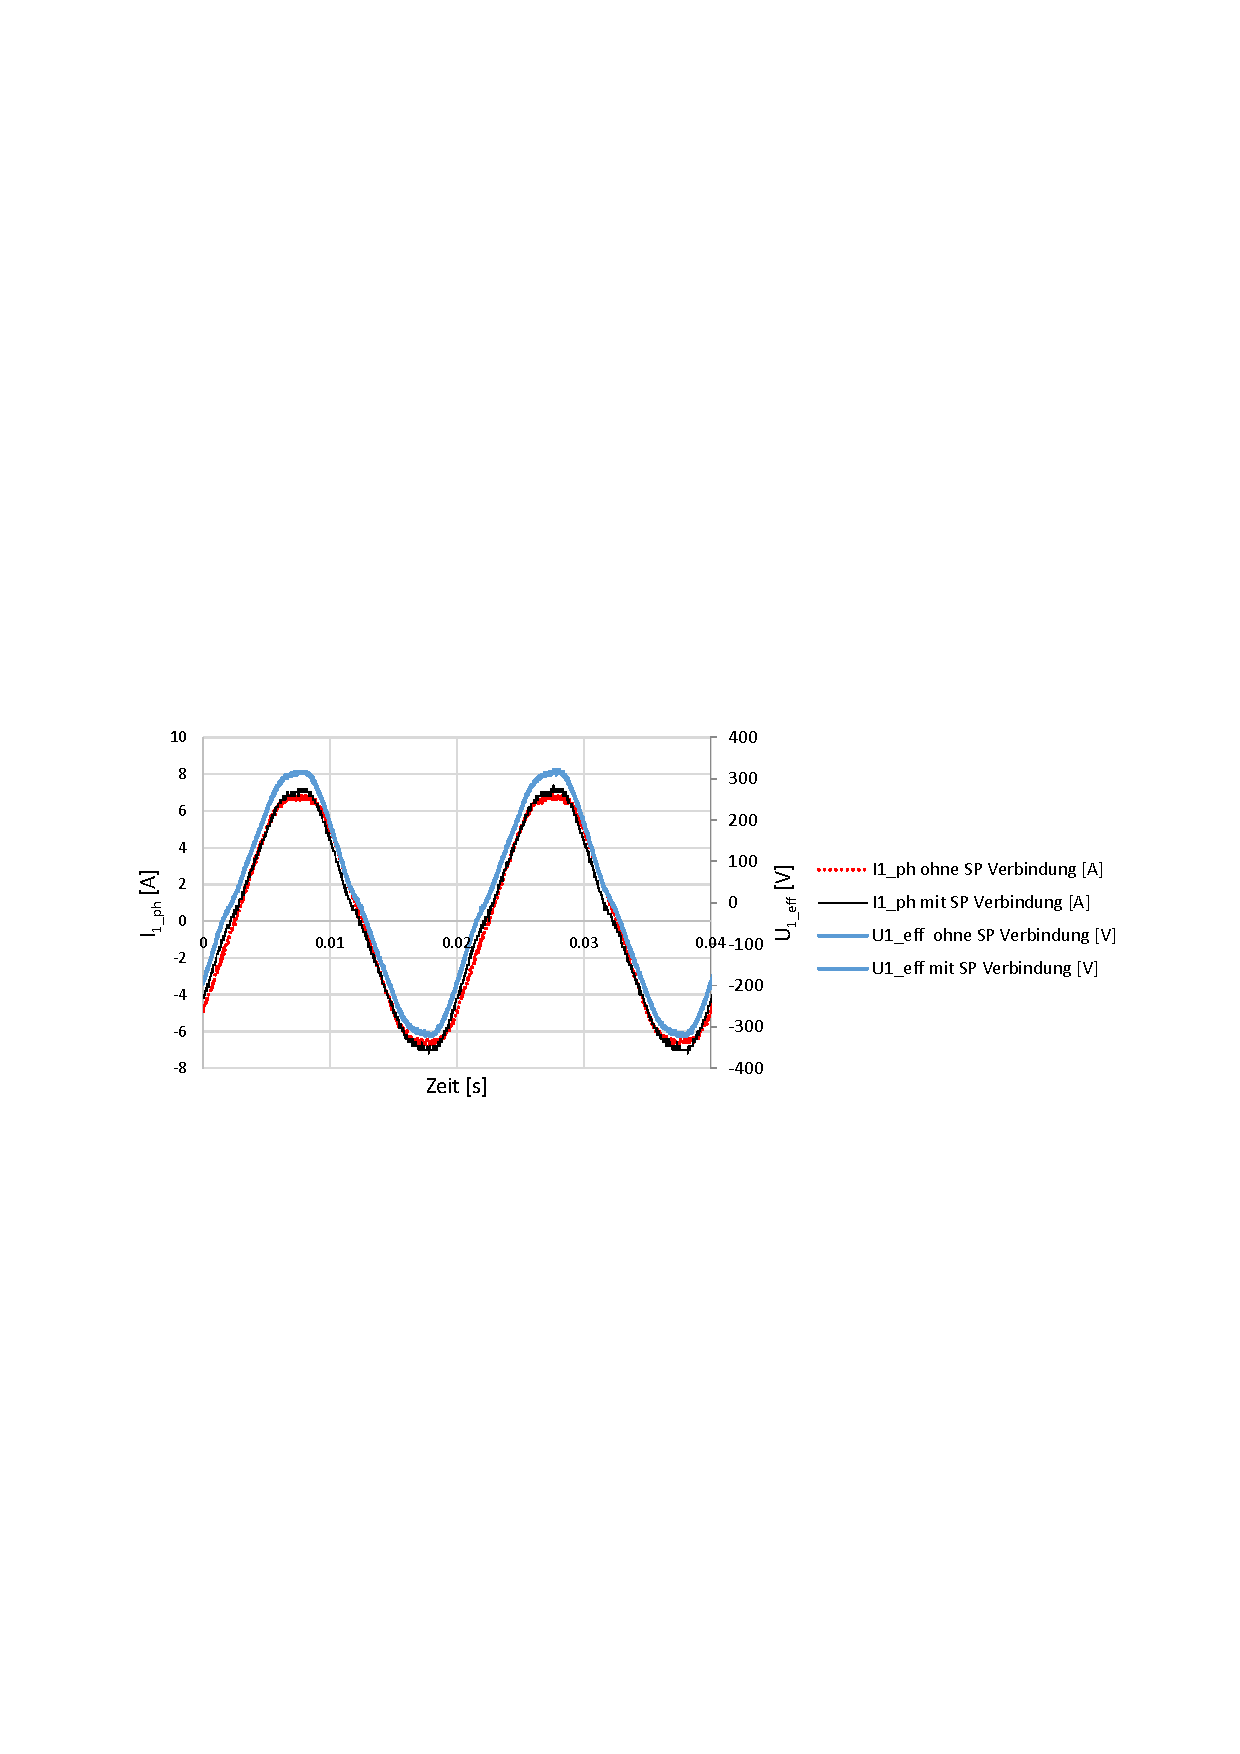
\includegraphics[ %trim=1cm 16.5cm 7.6cm 5.7cm, clip,
         width=\textwidth]{631_Bild7_Sternpunkt_MitOhneVerb.pdf}
    \caption{Einfluss Sternpunktbezug}
    \label{fig:EinflussSternpunktL}
\end{figure}
Bei Verbundenem Sternpunkt ändert sich der Strom $I_1$ kaum. Die verwendete Last verfügt also über eine gute Symmetrie.




\newpage
\subsection{Spannungsregelung}

In diesem Versuch wurde die Phasenspannung der SM über den Erregerstrom geregelt. So kann sichergestellt werden, dass die Statorspannung unabhängig der Last gleich bleibt.
Im Inselbetrieb, dh. wenn die SM als Generator betrieben wird, kann je nach Lastimpedanz die Spannung am Stator variieren. Da die Maschine in diesem Betriebszustand als Versorgungsnetz für andere elektrische Geräte dient, ist es wichtig, dass die Spannung konstant bleibt, unabhängig der zugeschalteten resp. weggeschalteten Lasten.\\
Die Regelung ist im Chopper integriert. \\

\vspace{0.3cm}



\begin{figure}[H]
    \centering
        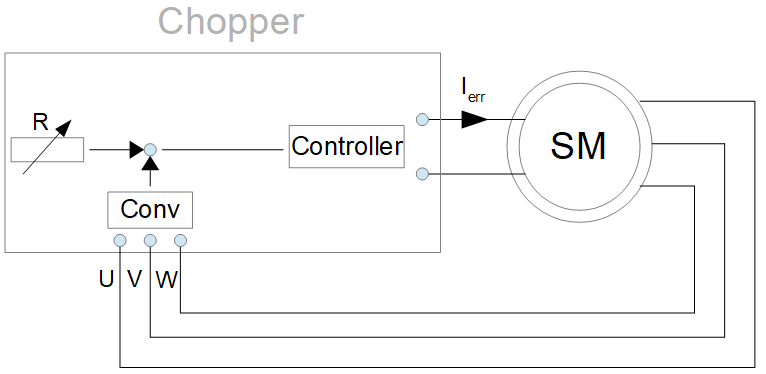
\includegraphics[ scale = 0.6]{632}
    \caption{Funktionsschema Spannungsregelung}
    \label{fig:shemaSpannungsregler}
\end{figure}



\subsubsection{Funktionsbeschreibung}
\vspace{0.3cm}
Über ein Potentiometer kann der Sollwert eingestellt werden. Diese Grösse, abzüglich dem Istwert definiert den Fehler. Über den Regler wird entsprechend die Stellgrösse, in diesem Fall der Erregerstrom $I_{err}$, angepasst. Grundsätzlich gilt; je höher der Erregerstrom, desto höher die Statorspannung. \\
Die Statorspannung wird zuerst konvertiert, damit sie mit der Sollgrösse verglichen werden kann.
%\textcolor{red}{evtl. KOnvertierungsmethode (Schema auf dem Chopper erklären - oder auch nicht :))}

\newpage


\subsubsection{Messung}
Die SM wurde für die Messung einem induktiven Laststoss ausgesetzt. In der Abbildung ist zu erkennen, dass der Regler die Spannung nach einem anfänglichen Überschwingen stabilisiert hat. Der Einschwingvorgang dauert ungefähr 2ms.\\

\vspace{0.5cm}



\begin{figure}[H]
    \centering
        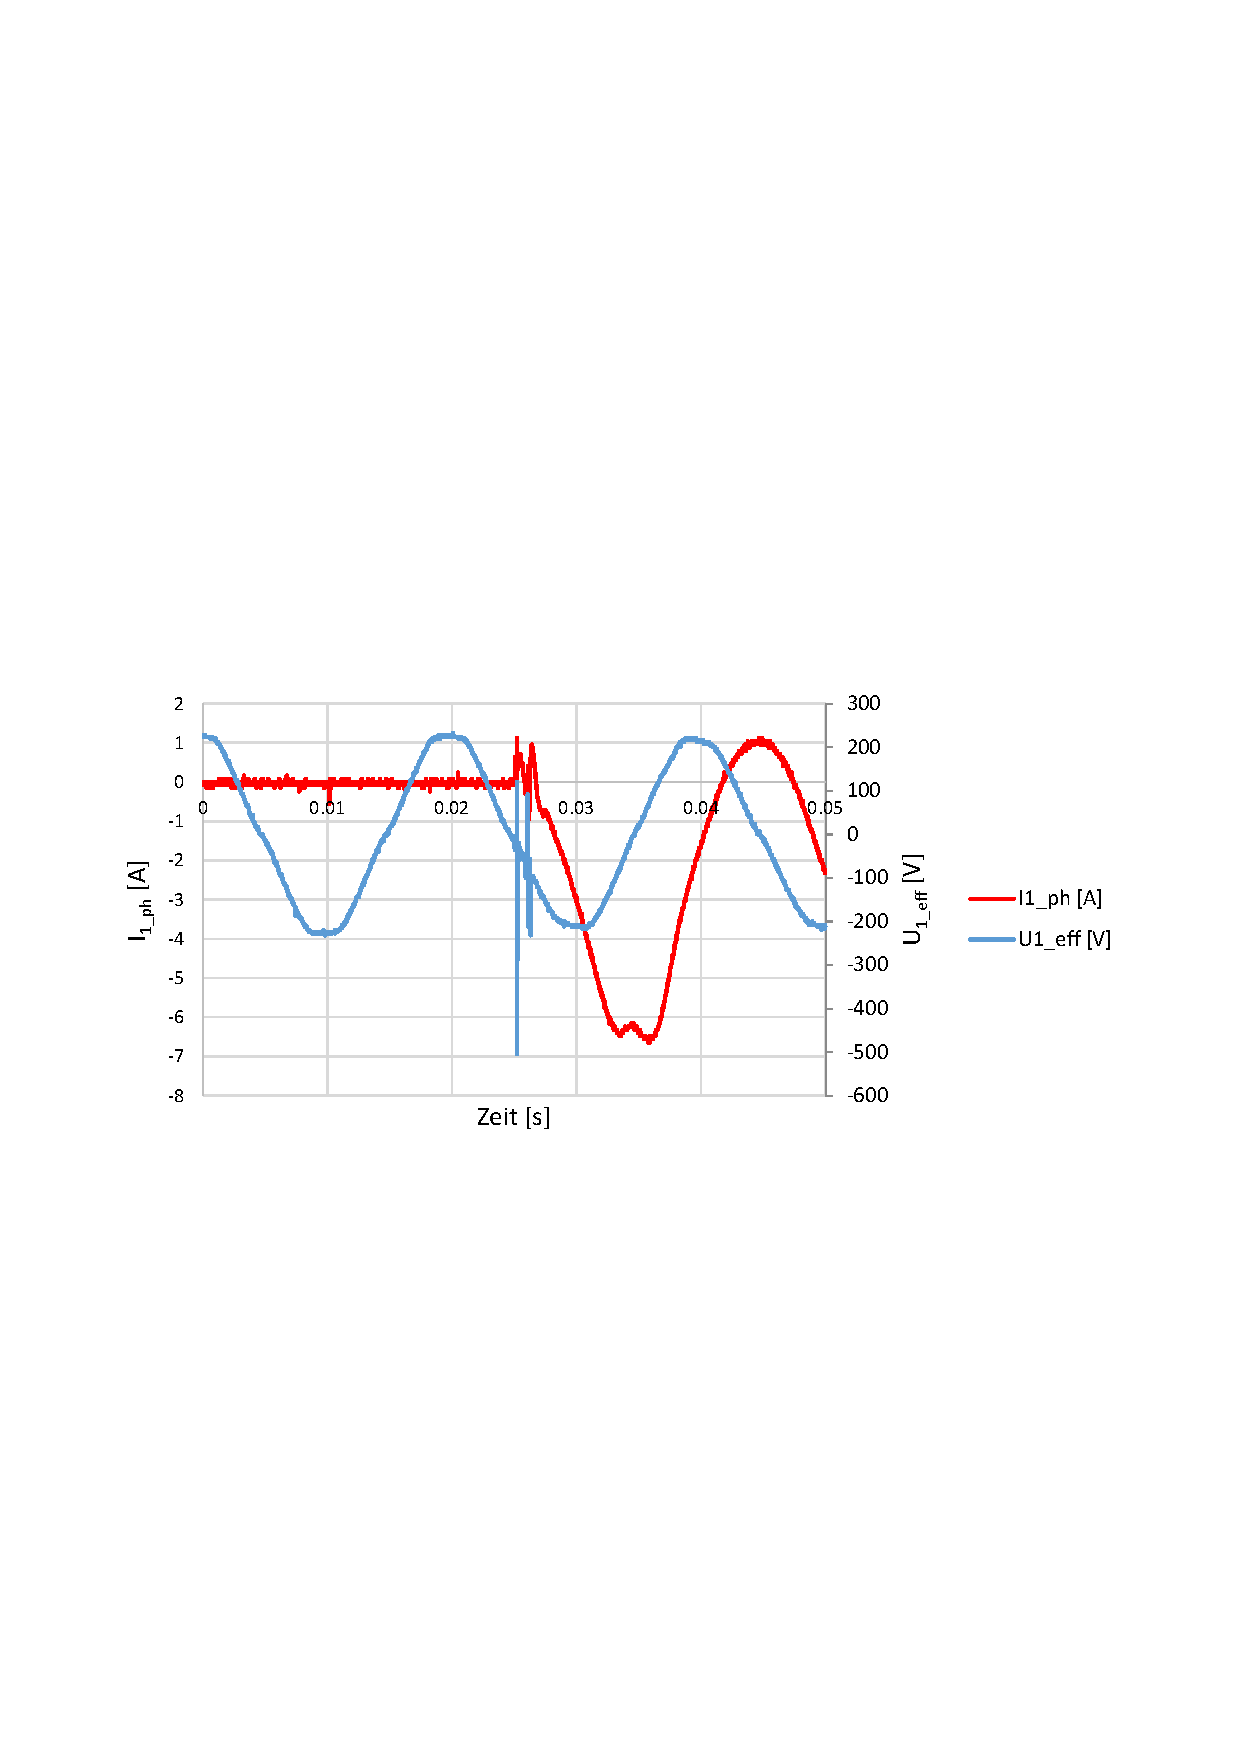
\includegraphics[ %trim=1cm 16.5cm 7.6cm 5.7cm, clip,
         width=\textwidth]{632_U-Regelung.pdf}
    \caption{Messung Spannungsregelung}
    \label{fig:MessungSpannungsregler}
\end{figure}






%\begin{figure}[ht!]
%    \captionsetup{justification=centering}
%\begin{minipage}[t]{0.26\textwidth}
%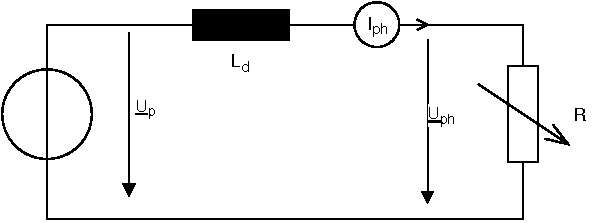
\includegraphics[width=\textwidth]{SM_Insel_1PH_R.pdf}
%\subcaption{Ohmsche Last}
%\label{fig:abb1}
%\end{minipage}
%\begin{minipage}[t]{0.37\textwidth}
%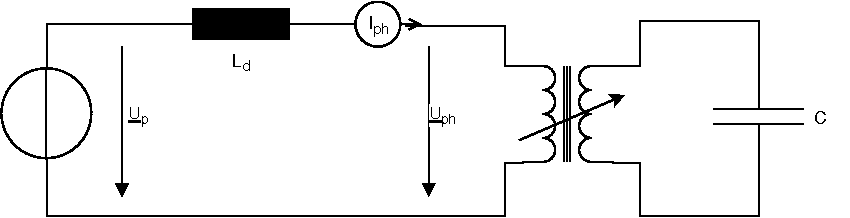
\includegraphics[width=\textwidth]{SM_Insel_1PH_C.pdf}
%\subcaption{Kapazitive Last}
%    \label{fig:abb1}
%\end{minipage}
%\begin{minipage}[t]{0.37\textwidth}
%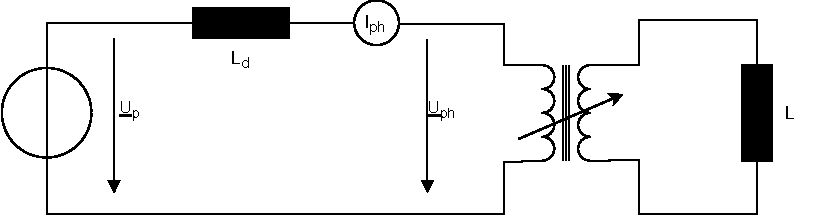
\includegraphics[width=\textwidth]{SM_Insel_1PH_L.pdf}
%\subcaption{Induktive Last}
%    \label{fig:abb1}
%\end{minipage}
%\caption{Einphasen Ersatzschaltbild der SM im Inselbetrieb}
%\end{figure}




%\begin{figure}[ht!]
%    \captionsetup{justification=centering}
%\begin{minipage}[t]{0.32\textwidth}
%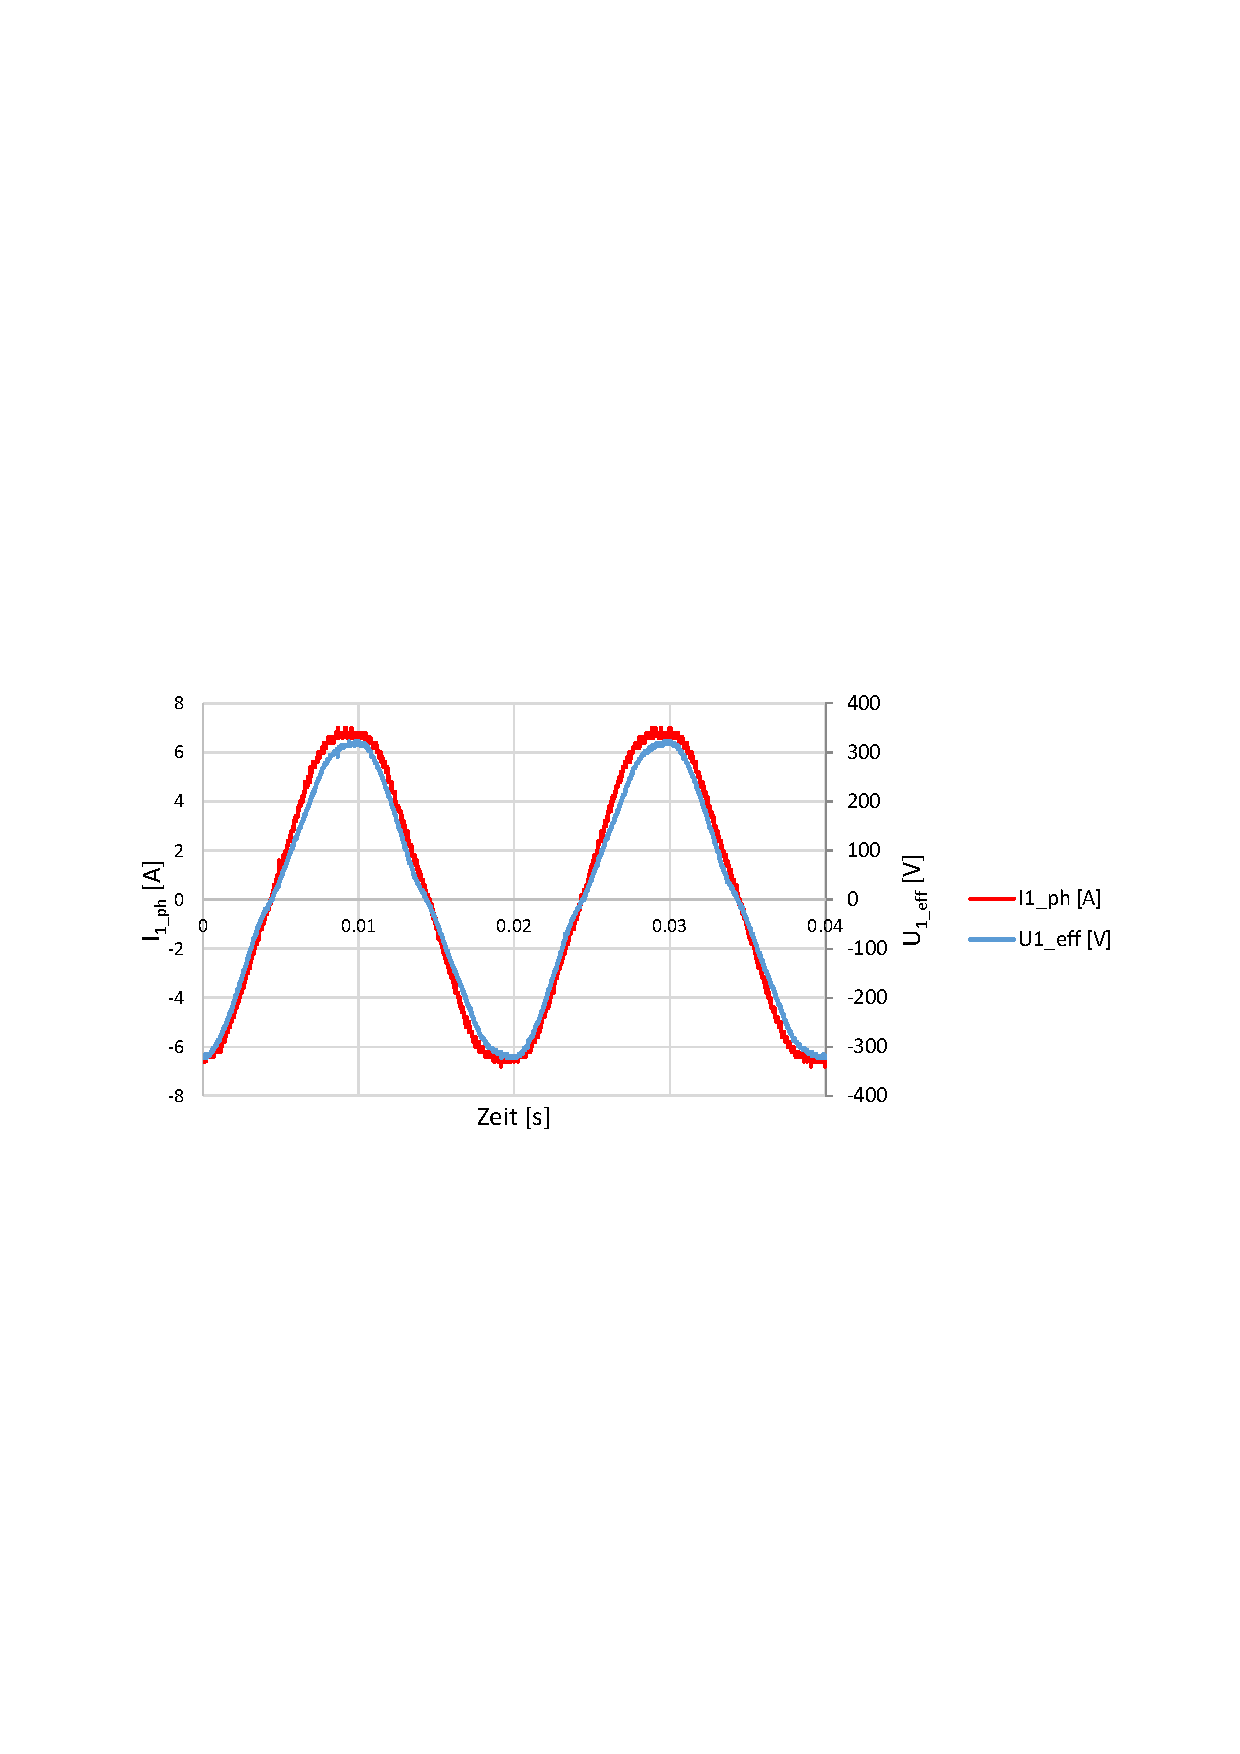
\includegraphics[width=\textwidth]{631_Bild4_Ohmsch.pdf}
%\subcaption{Ohmsche Last}
%\label{fig:abb1}
%\end{minipage}
%\begin{minipage}[t]{0.32\textwidth}
%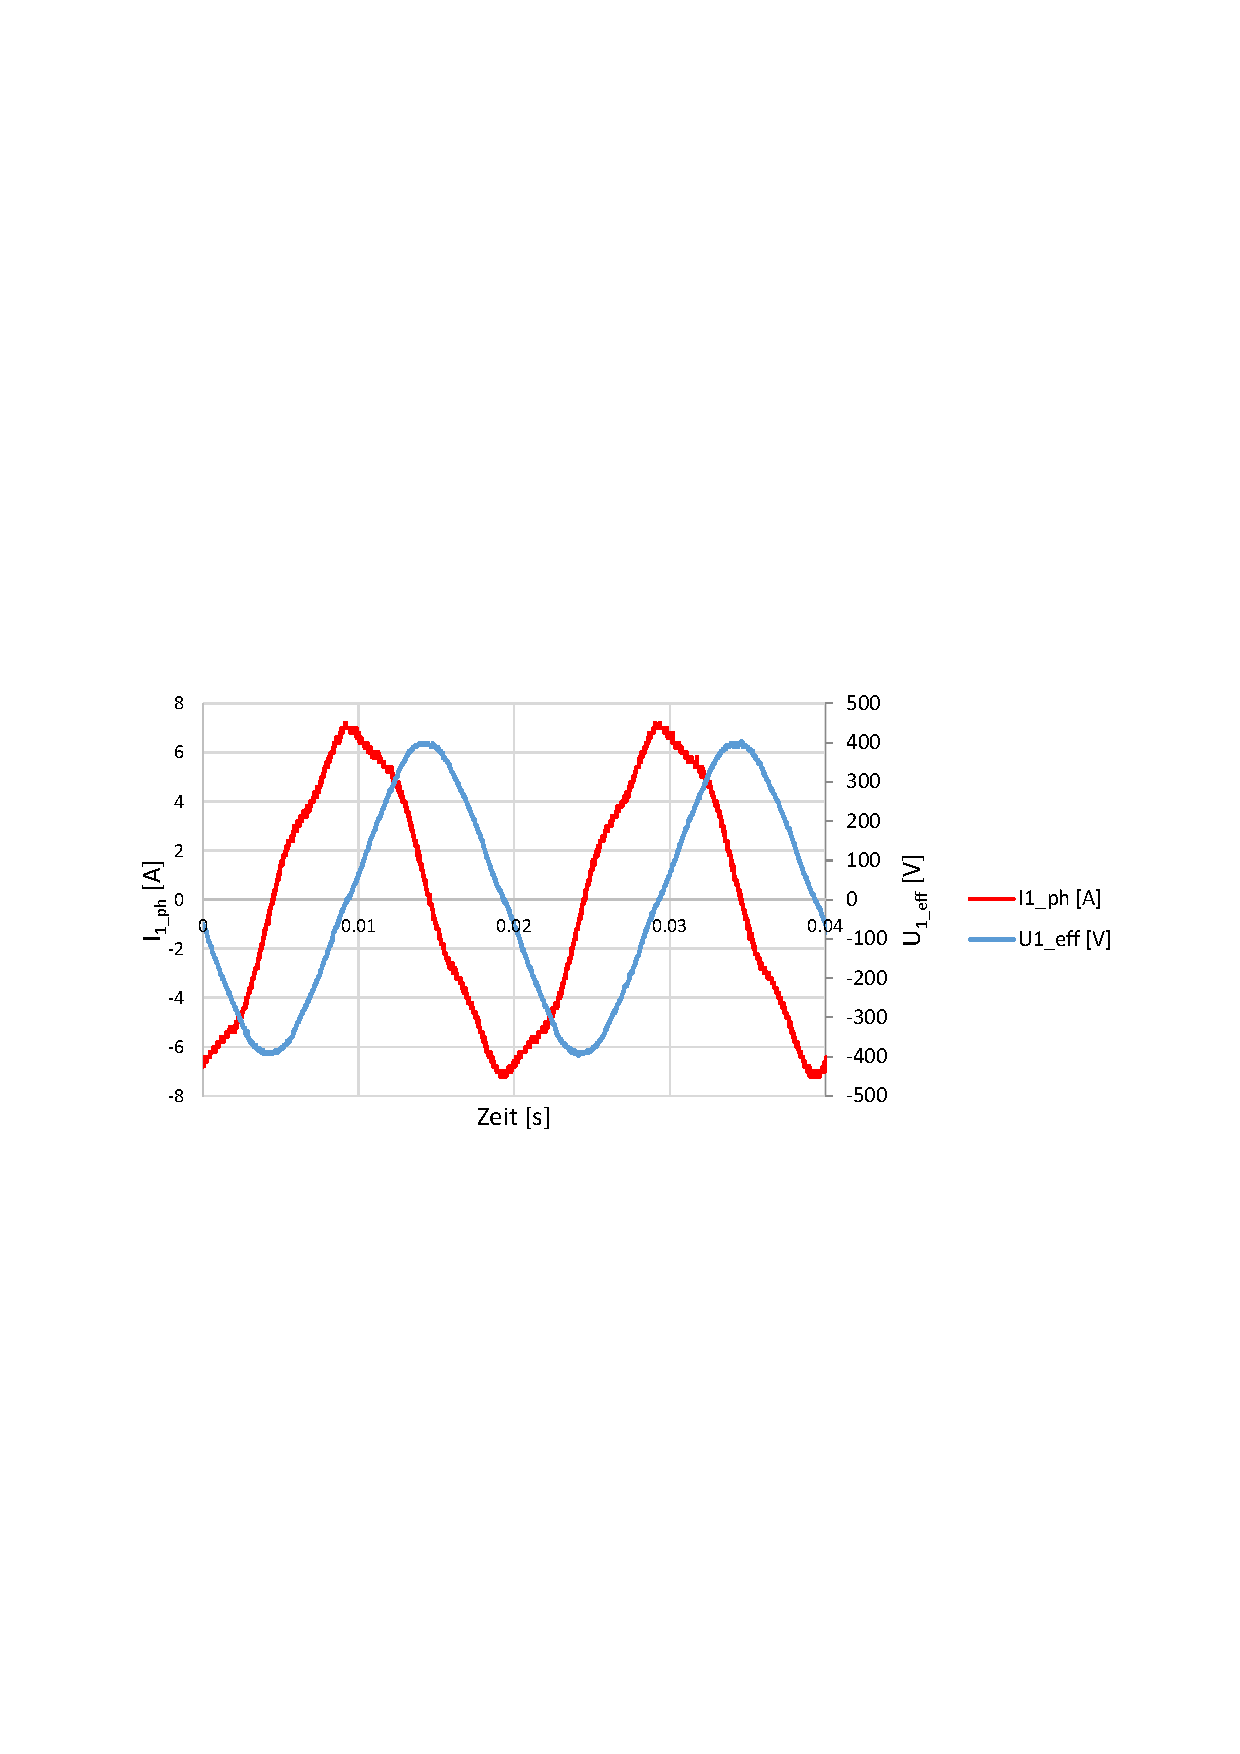
\includegraphics[width=\textwidth]{631_Bild5_Kapazitiv.pdf}
%\subcaption{Kapazitive Last}
%    \label{fig:abb1}
%\end{minipage}
%\begin{minipage}[t]{0.32\textwidth}
%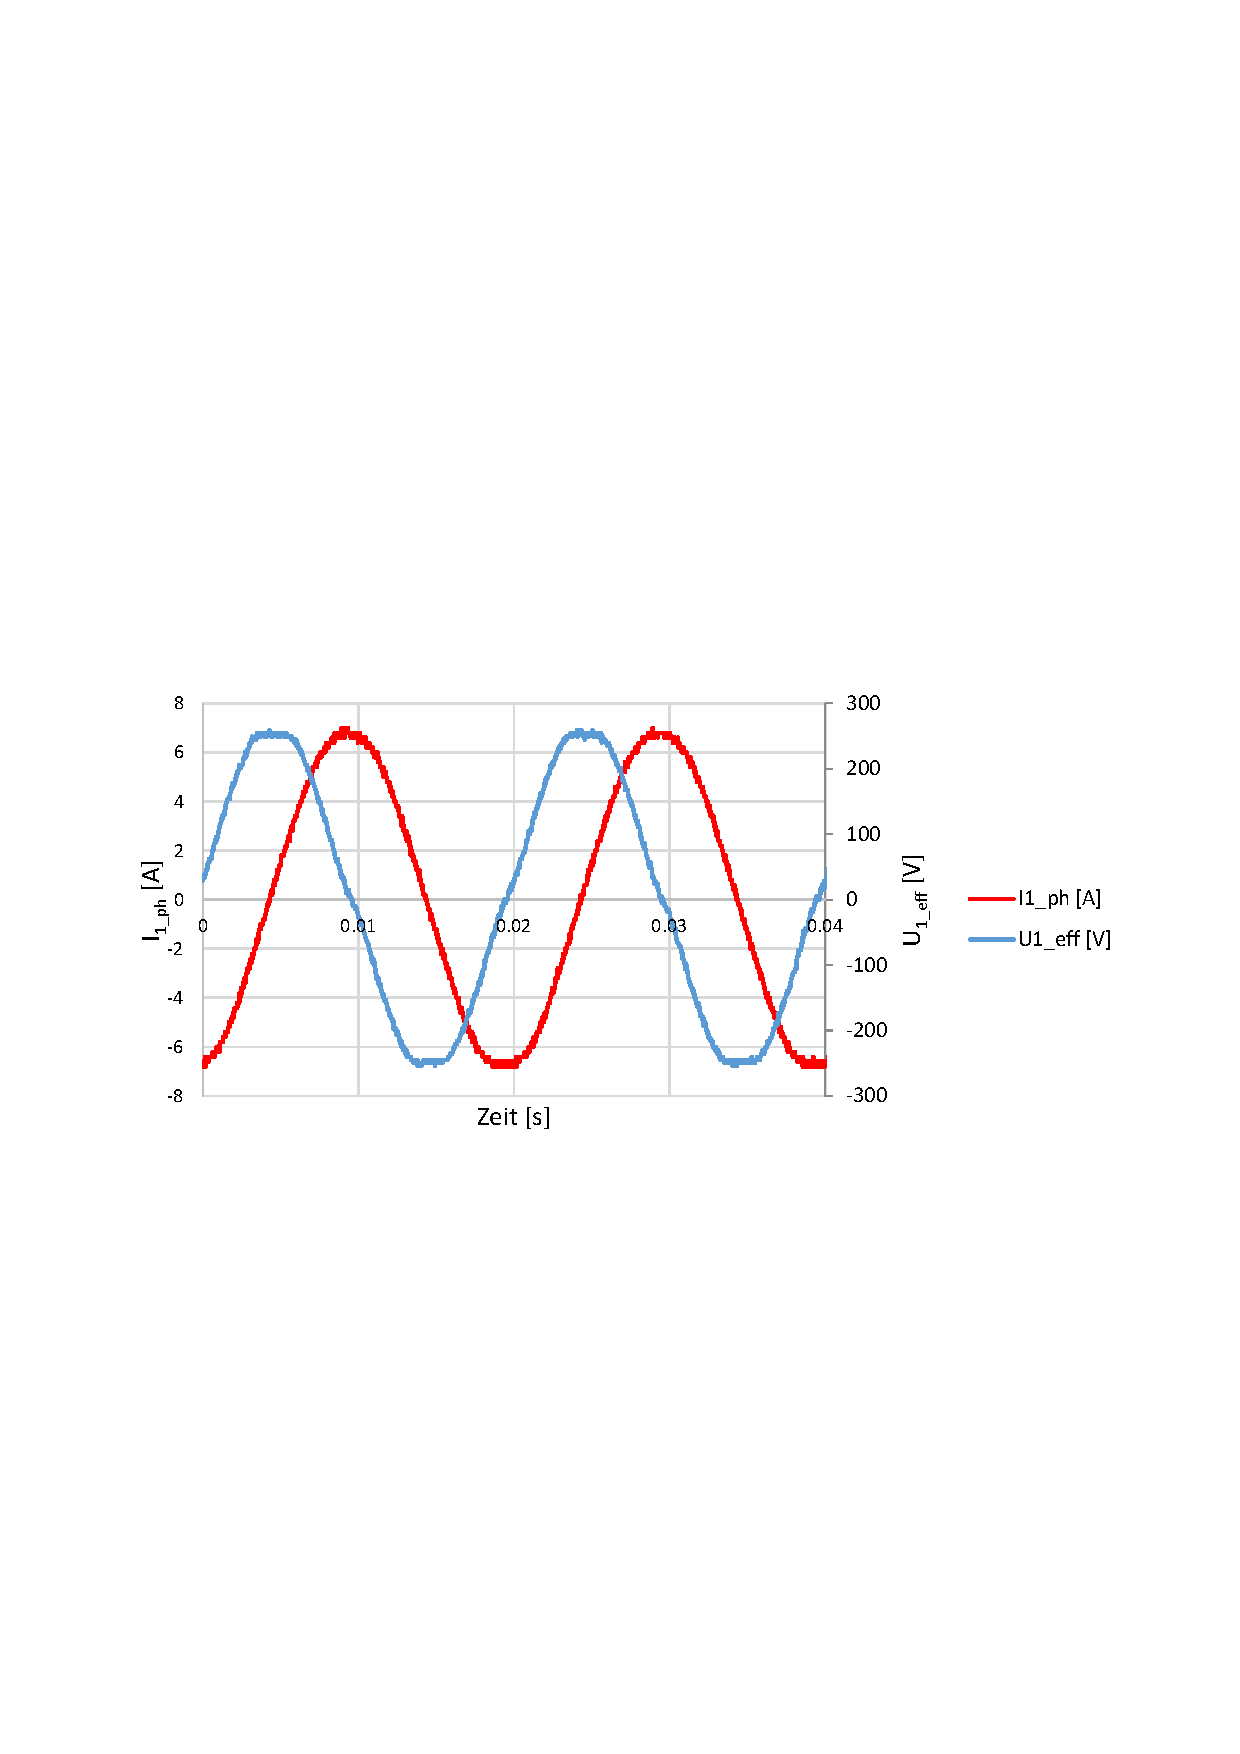
\includegraphics[width=\textwidth]{631_Bild6_Induktiv.pdf}
%\subcaption{Induktive Last}
%    \label{fig:abb1}
%\end{minipage}
%\caption{Verlauf des Phasenstom und der Spannung}
%\end{figure}


\newpage
\addtocontents{toc}{\protect\newpage}  % seitenumbruch im Inhaltsverzeichnis erzwingen
\section{SM am Netz}\label{netz}

\vspace{0.3cm}
\begin{figure}[H]
    \centering
        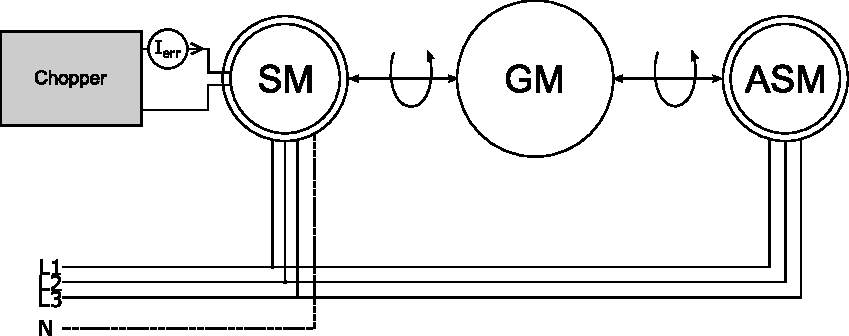
\includegraphics[width=\textwidth]{SM_Netzbetrieb_Uebersicht.pdf}
    \caption{Übersicht SM am Netz}
    \label{fig:SMNetz}
\end{figure}\vspace{0.3cm}
 Bei diesem Versuch läuft die Synchronmaschine direkt am Netz. Dazu muss sie zuerst synchronisiert werden. 

\subsection{Synchronisation}
Der Asynchronmotor mit einem Widerstand im Rottorkreis Treibt die Welle auf rund 1490 $\frac{1}{min}$. Danach dient die Gleichstrommaschine zum erhöhen auf 1500 $\frac{1}{min}$. Nach dem die Ausgangsspannung der Synchronmaschine $U_1$ über den Erregerstrom an die Netzspannung $U_{L1}$ angepasst ist, erfolgt über das Moment der Gleichstrommaschine das Angleichen der Phasenlage von $U_1$ an $U_{L1}$. Das Synchronoskop zeigt die Differenz der beiden an. Bei Synchronlauf werden sie zusammen geschaltet. 
\vspace{0.3cm}
\begin{figure}[H]
    \centering
        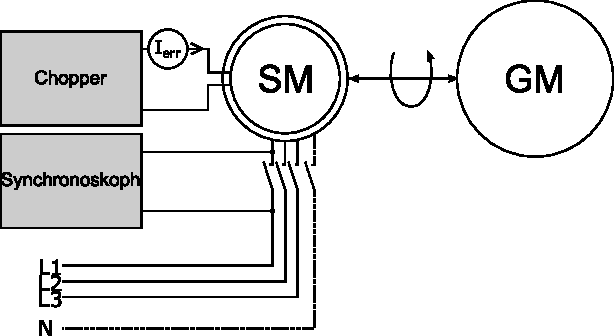
\includegraphics[width=0.6\textwidth]{SM_Synchronisation.pdf}
    \caption{Darstellung der Synchronisation}
    \label{fig:Synchronisation}
\end{figure}\vspace{0.3cm}
\subsubsection{Verbinden des Nulleiter}
Bei verbundenem Nulleiter kann man gut die Abweichung Zwischen der Netzspannung und der Synchronmaschinenausgangsspannung erkennen. Die Unterschiede entstehen, weil die Maschine nicht absolut symmetrisch gewickelt ist. Am deutlichsten zeigt sich der Anteil einer dritten Harmonischen im Strom der Sternpunktverbindung. Im Gegensatz dazu verläuft der Phasenstrom ohne Sternpunktverbindung nahezu sinusförmig.


\begin{figure}[H]
\begin{minipage}[t]{0.49\textwidth}
\centering
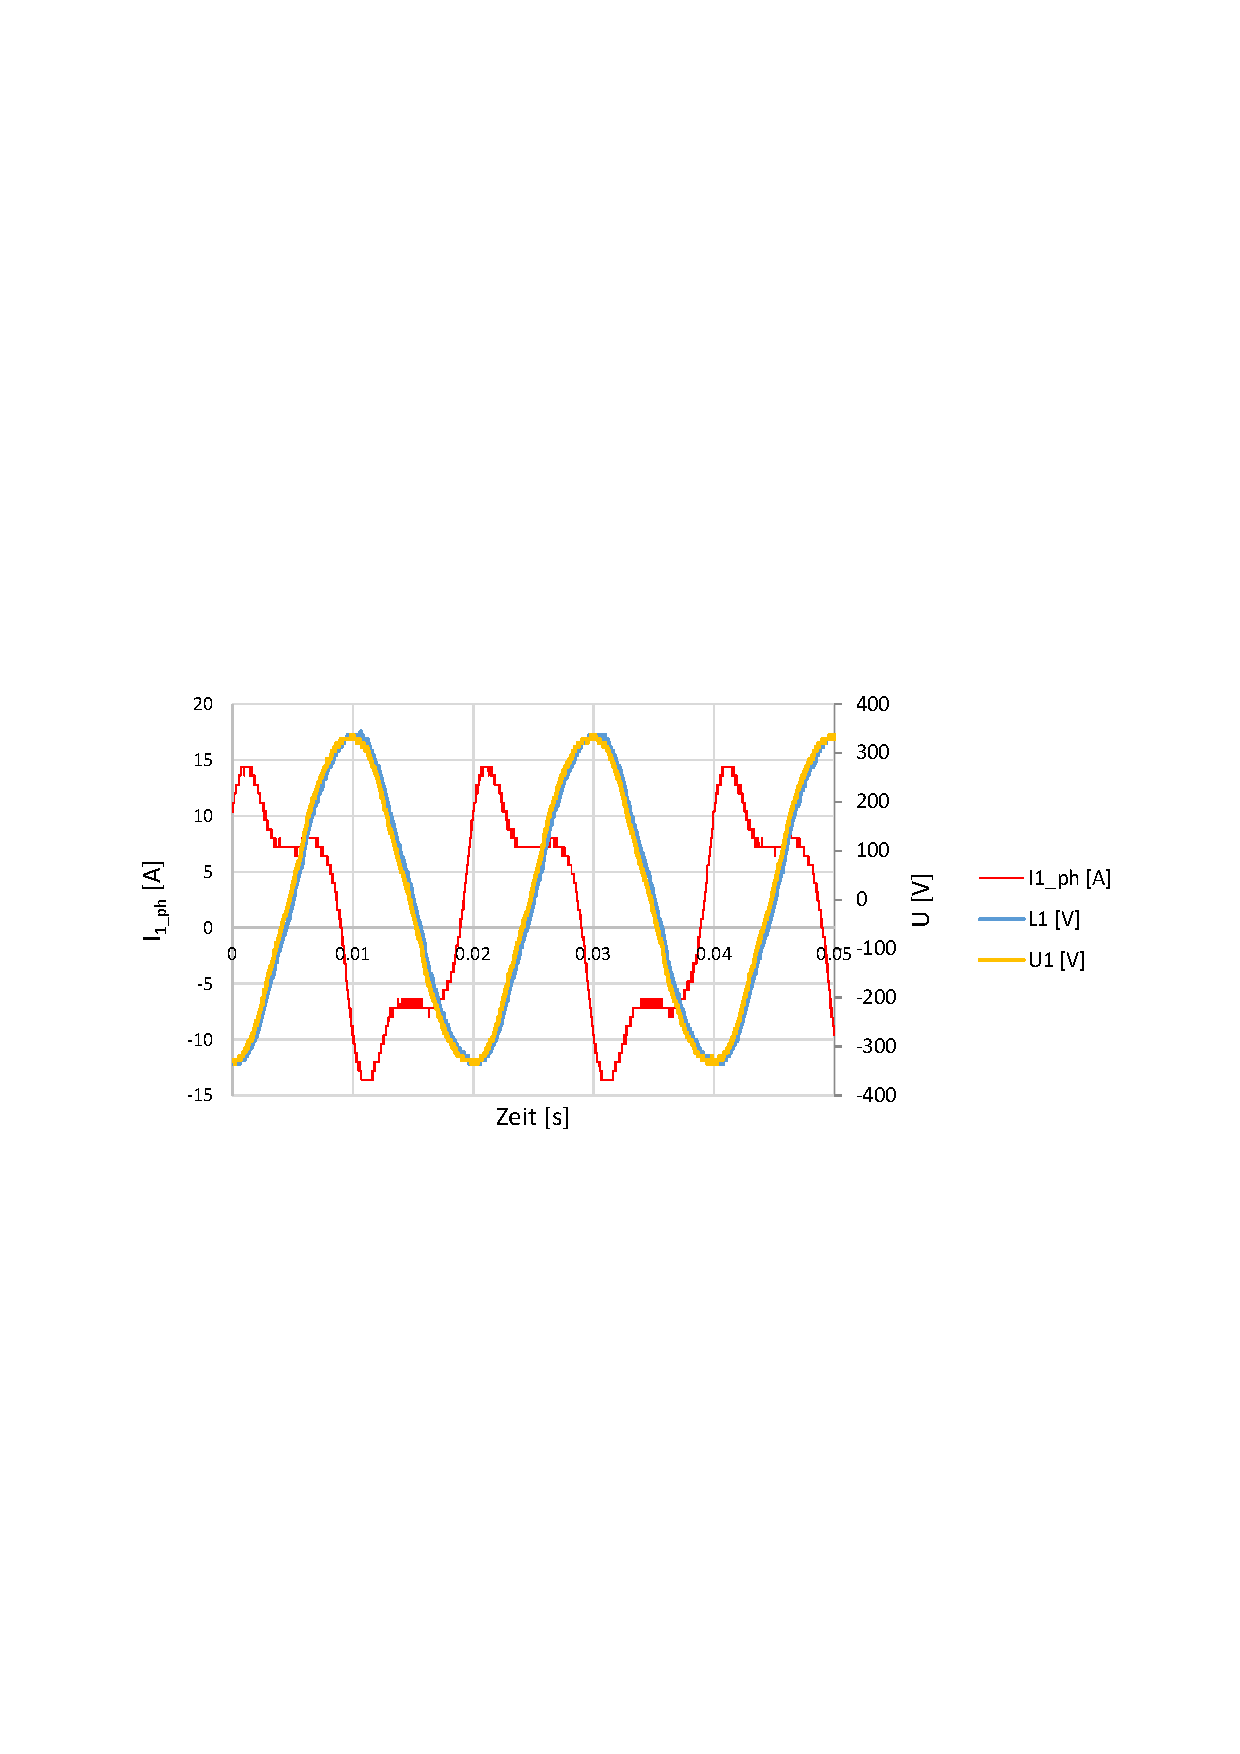
\includegraphics[trim=0cm 5cm 0cm 5cm, clip,
width=\textwidth]{641_Bild5_PhasenstromBeiSternpunktverbindung.pdf}
\subcaption{Phasenstrom}
\label{fig:PhasenstromSternpuntkverbunden}
\end{minipage}
\begin{minipage}[t]{0.49\textwidth}
\centering
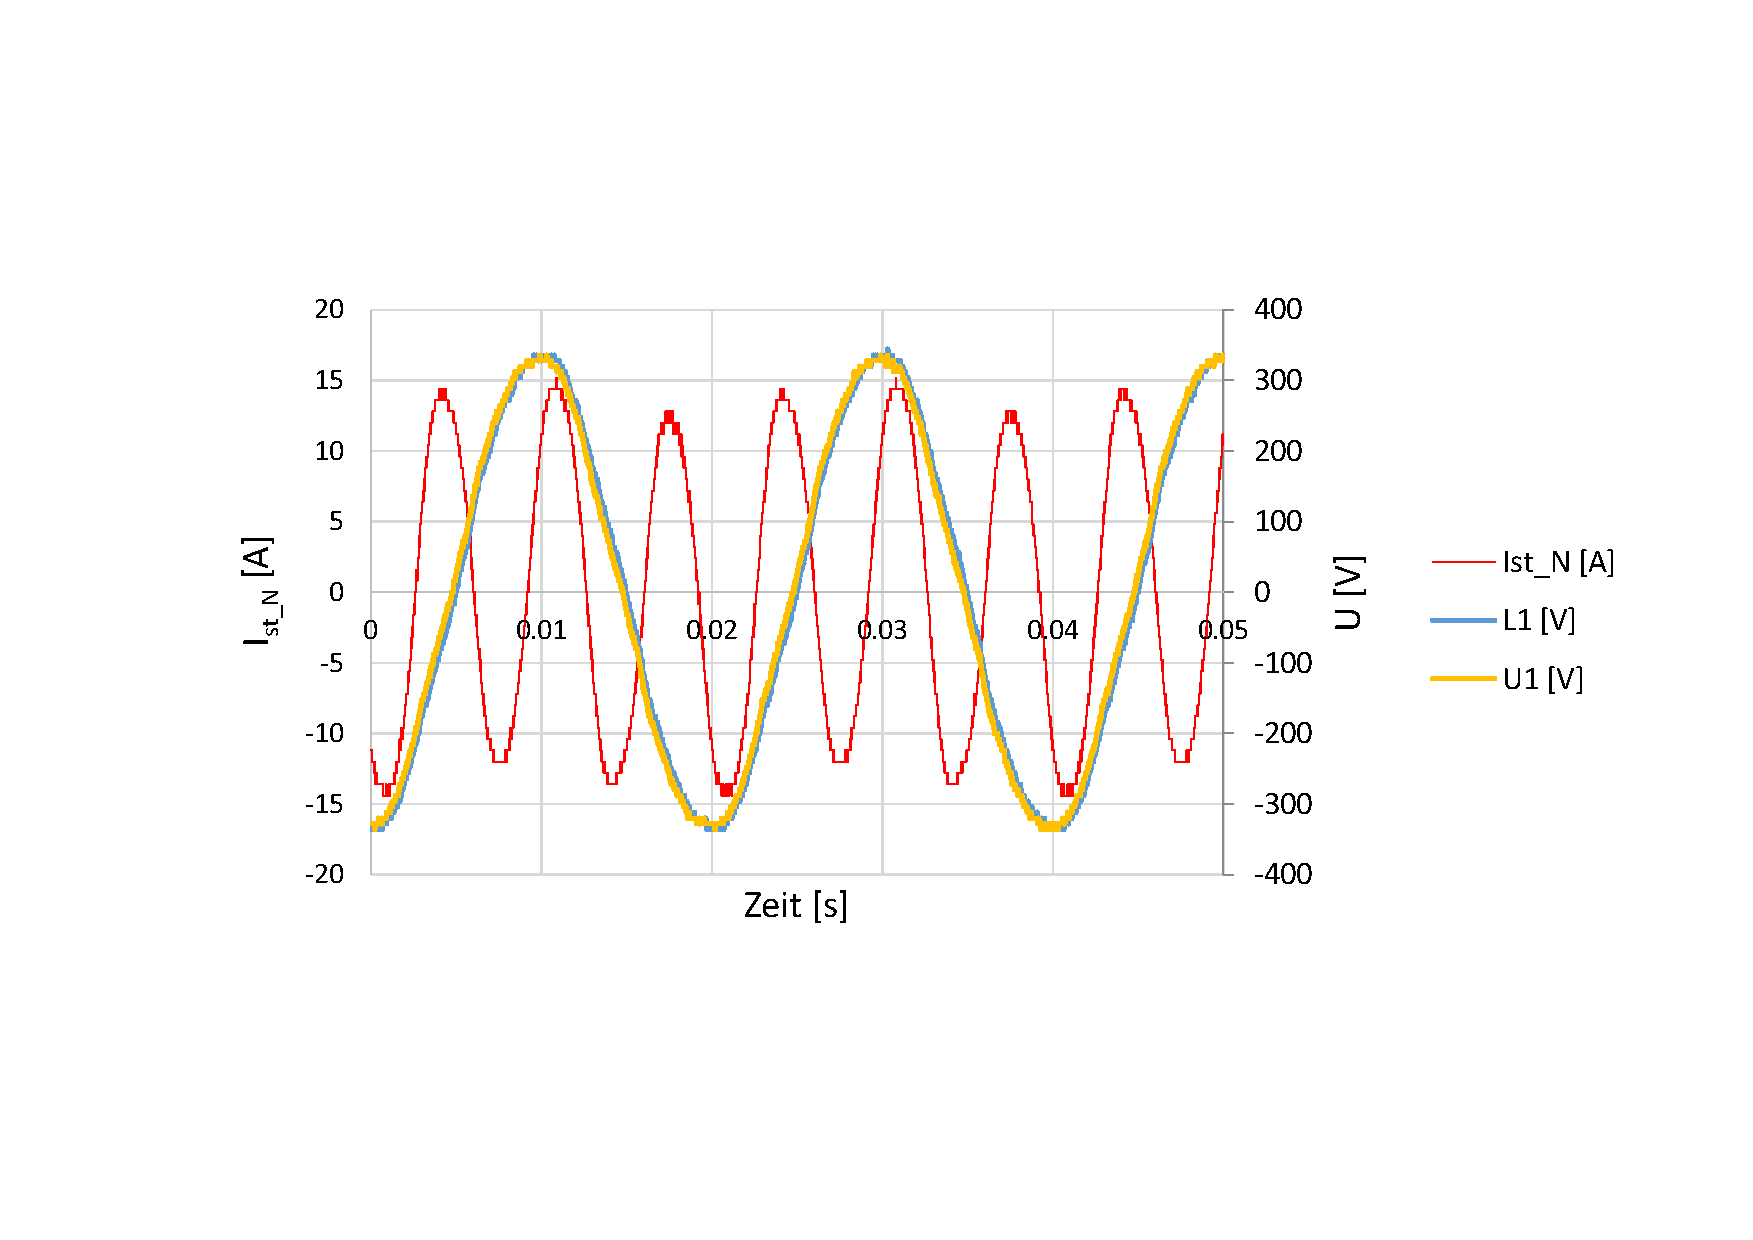
\includegraphics[trim=0cm 5cm 0cm 5cm, clip,
width=\textwidth]{641_Bild4_Nulleiterstrom}
\subcaption{Strom in der Sternpunktverbindung}
    \label{fig:SternstromVerbunden}
\end{minipage}
\caption{Strom und Spannung bei verbundenen Sternpunkten}
\end{figure}





\subsection{Dämpferwicklung}

In nächsten Versuch läuft die Asynchronmaschine als Dämpferwicklung mit. Sie dämpft Schwingungen die durch starke Laständerungen oder bei Zuschalten eines nicht ganz synchron laufenden Netzes entstehen. Eine Strommessung im Rotorkreis der ASM zeigt das Verhalten.
\vspace{0.3cm}
\begin{figure}[H]
    \centering
    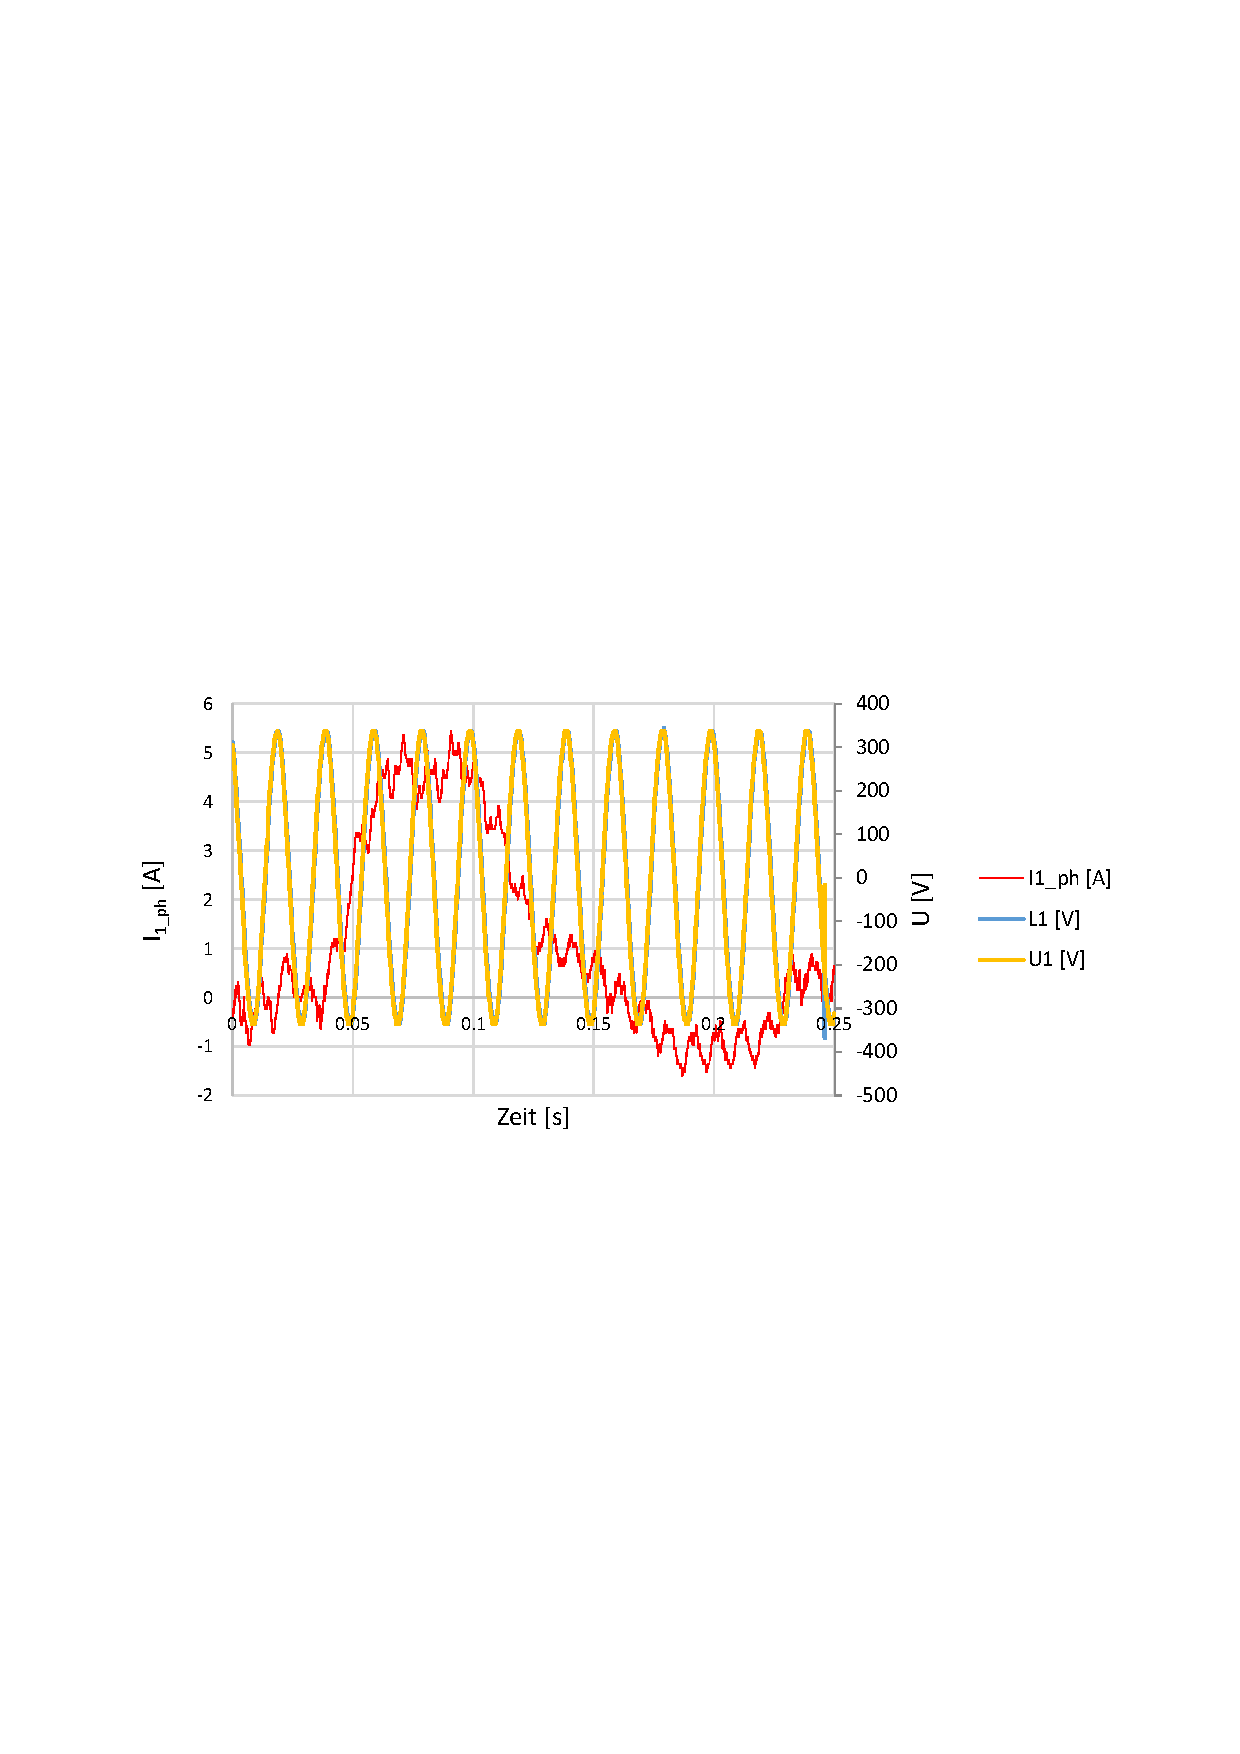
\includegraphics[width=0.8\textwidth]{641_Bild2_LastabwurfKurzgeschlossen}
    \caption{Rotorstrom der ASM bei kurzgeschlossenem Rotor}
    \label{fig:RotorstromUnGedampft}
\end{figure}\vspace{0.3cm}
Deutlich ist sichtbar, wie der Strom bei einem Lastabwurf kurzzeitig ansteigt und sich dann schnell wieder um 0 einpändelt. Anders sieht es aus nach der Reduktion der Dämpfung durch einen Widerstand am Rotor der ASM. 

\vspace{0.3cm}
\begin{figure}[H]
    \centering
		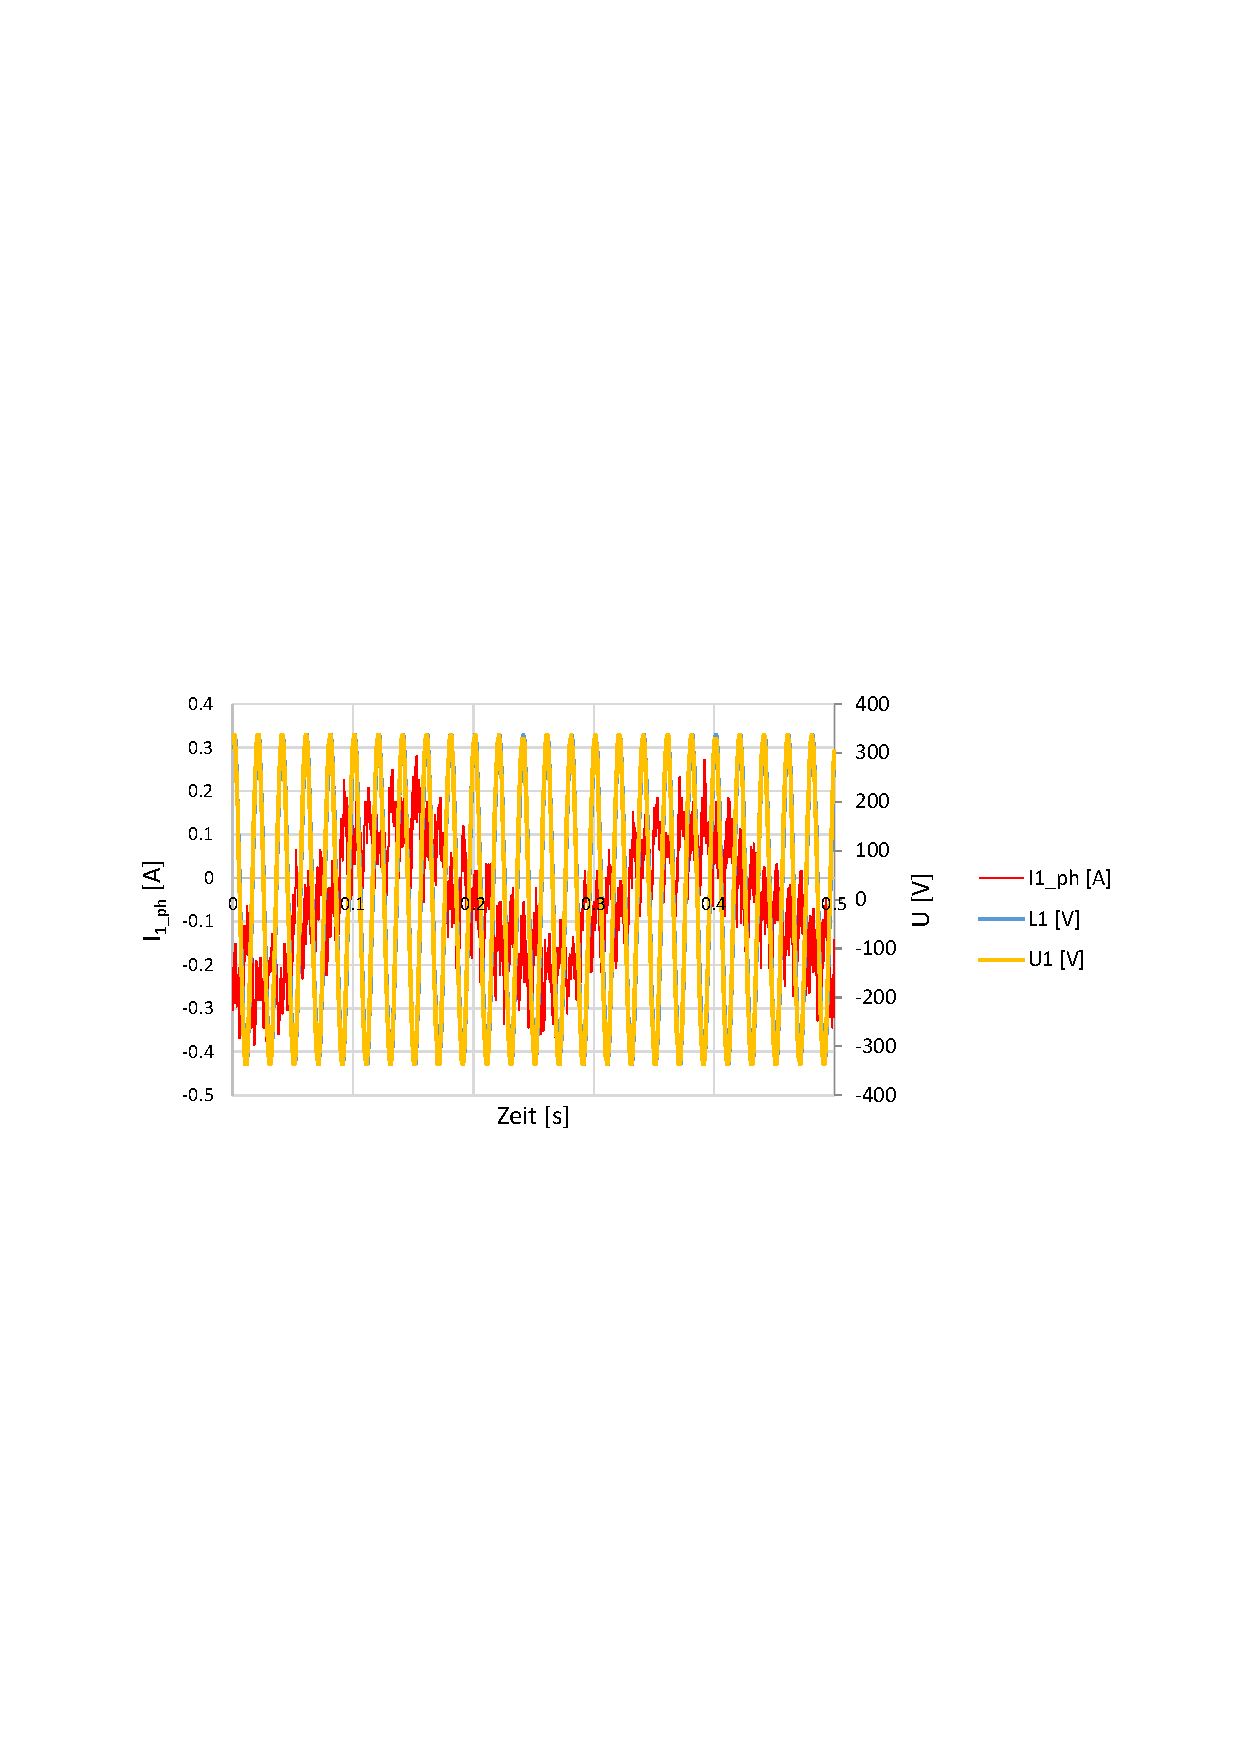
\includegraphics[width=0.8\textwidth]{641_Bild3_LastabwurfWiderstand}
    \caption{Rotorstrom der ASM bei Widerstand am Rotor}
    \label{fig:RotorstromGedampft}
\end{figure}\vspace{0.3cm}
Die im Strom sichtbaren Schwingungen sind auch gut hör- und spürbar.

\newpage
\subsection{Variation der Wirkleistung}
Für diesen Versuchsaufbau wurde die SM mit einem Nennerregerstrom von 1.1A betrieben. Durch die Variation der Last (Drehmoment der GM) soll veranschaulicht werden, wie sich der Polradwinkel in Abhängigkeit der Last verändert.\\

\vspace{0.8cm}


\begin{tabular}{|l|l|l|l|l|l|}
 \hline
 \rowcolor[gray]{.8}  $M$ [Nm] &  $\varphi$ [\degree]&  $S_1$  [kVA]&$P_1$ [kW]& $I_1$ [A] &Bemerkung\\
\hline
\hline
 -10 & -2.2 & 0.51 & 0.5& 2.2& -\\
\hline
 -20 & -5.3 & 1.035 & 1.03& 4.4  & -\\
\hline
-30& -8.8 & 1.56 & 1.55 & 6.7 &-\\
\hline
\end{tabular}




\textcolor{red}{TODO\\-Zeigerdiagramme Skizzieren\\-Erkenntnisse beschreiben}


\newpage
\subsection{Variation der Blindleistung}

Für diesen Versuch wurde die ASM elektrisch entkoppelt (Rotorkreis offen).Über den Erregerstrom der SM wurde die Blindleistung variert. Je nach Betriebsfall (unter-/bzw. übererregt) fällt die Blindleistung positiv oder negativ aus.\\
\vspace{0.8cm}


\begin{tabular}{|l|l|l|l|l|l|l|}
 \hline
 \rowcolor[gray]{.8} $I_{err}$ [A] & $M$ [Nm] &  $\varphi$ [\degree]&  $S_1$  [kVA]&$P_1$ [kW]& $I_1$ [A] &Bemerkung\\
\hline
\hline
 0.5&-20.3 & -7.6 & 2.77 & 1.12& 11.8& $Q$ positiv\\
\hline
 0.8&-20.3 & -6 & 1.73 & 1.06& 7.4  & $Q$ positiv\\
\hline
\hline
\rowcolor[gray]{.9} 1.1&-20.3& -5.4 & 1.05 & 1.04& 4.5 &Nennbetrieb \\
\hline
\hline
1.5&-20.3&-5&1.76&1.07&7.2&$Q$ negativ\\
\hline
1.8&-20.4&-5&2.78&1.1&11.9&$Q$ negativ\\
\hline
\end{tabular}



\textcolor{red}{TODO\\-Zeigerdiagramme skizzieren \\-V-Kurve (I1 in abhängigkeit von Ierr) Skizzieren (bei 0.5kW und 5kW)\\-Erkenntnisse\\-Blindleistung berechnen mit Wattmeter: https://de.wikipedia.org/wiki/Blindleistung --> Unten bei \textbf{Symmetrische Belastung}}





\end{flushleft}